\chapter*{Vorwort}
Dieses Skript wird/wurde im Wintersemester 2013/2014
von Martin Thoma geschrieben. Es beinhaltet die Mitschriften aus
der Vorlesung von Prof. Dr. Herrlich sowie die Mitschriften einiger
Übungen und Tutorien.

An dieser Stelle möchte ich Herrn~Prof.~Dr.~Herrlich für einige 
Korrekturvorschläge und einen gut strukturierten Tafelanschrieb 
danken, der als Vorlage für dieses Skript diente. Tatsächlich basiert
die Struktur dieses Skripts auf der Vorlesung von Herrn~Prof.~Dr.~Herrlich
und ganze Abschnitte konnten direkt mit \LaTeX{} umgesetzt werden.
Vielen Dank für die Erlaubnis, Ihre Inhalte in diesem Skript einbauen
zu dürfen!

Vielen Dank auch an Frau Lenz und Frau Randecker, die es mir erlaubt 
haben, ihre Übungsaufgaben und Lösungen zu benutzen.

Das Skript ist kostenlos über \href{http://martin-thoma.com/geotopo/}{martin-thoma.com/geotopo}
verfügbar. Wer es gerne in A5 (Schwarz-Weiß, Klebebindung) für ca. 10 Euro hätte, 
kann mir eine Email schicken (info@martin-thoma.de).

\section*{Was ist Topologie?}

Die Kugeloberfläche $S^2$ lässt sich durch strecken, stauchen
und umformen zur Würfeloberfläche oder
der Oberfläche einer Pyramide verformen, aber nicht zum $\mdr^2$
oder zu einem Torus $T^2$. Für den $\mdr^2$ müsste man die Oberfläche
unendlich ausdehnen und für einen Torus müsste man ein Loch machen.

\begin{figure}[ht]
    \centering
    \subfloat[$S^2$]{
        % Source: http://tex.stackexchange.com/a/42865/5645
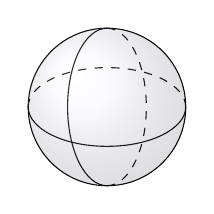
\begin{tikzpicture}
    \draw (-1,0) arc (180:360:1cm and 0.5cm);
    \draw[dashed] (-1,0) arc (180:0:1cm and 0.5cm);
    \draw (0,1) arc (90:270:0.5cm and 1cm);
    \draw[dashed] (0,1) arc (90:-90:0.5cm and 1cm);
    \draw (0,0) circle (1cm);
    \shade[ball color=blue!10!white,opacity=0.20] (0,0) circle (1cm);
\end{tikzpicture}

        \label{fig:s2}
    }%
    \subfloat[Würfel]{
        % Source: http://tex.stackexchange.com/a/12069/5645
\begin{tikzpicture}[scale=0.5]
   \clip (-3,-3) rectangle (3,3);
   \coordinate (tf) at (0,0);
   \coordinate (bf) at (0,-3);
   \coordinate (tr) at (15:2.5cm);
   \coordinate (tl) at (165:2.5cm);

   % You can change the perspective by playing with the 5, 5, 15:
   \coordinate (fr) at ($ (tf)!5!(tr) $);
   \coordinate (fl) at ($ (tf)!5!(tl) $);
   \coordinate (fb) at ($ (tf)!15!(bf) $);

   \path[name path=brpath] (bf) -- (fr);
   \path[name path=rbpath] (tr) -- (fb);
   \path[name path=blpath] (bf) -- (fl);
   \path[name path=lbpath] (tl) -- (fb);
   \path[name path=trpath] (tl) -- (fr);
   \path[name path=tlpath] (tr) -- (fl);

   \draw[name intersections={of=brpath and rbpath}] (intersection-1)coordinate (br){}; 
   \draw[name intersections={of=blpath and lbpath}] (intersection-1)coordinate (bl){}; 
   \draw[name intersections={of=trpath and tlpath}] (intersection-1)coordinate (tb){}; 

   \shade[right color=gray!10, left color=black!50, shading angle=105] (tf) -- (bf) -- (bl) -- (tl) -- cycle;
   \shade[left color=gray!10, right color=black!50, shading angle=75] (tf) -- (bf) -- (br) -- (tr) -- cycle;

   \begin{scope}
      \clip (tf) -- (tr) -- (tb) -- (tl) -- cycle;
      \shade[inner color = gray!5, outer color=black!50, shading=radial] (tf) ellipse (3cm and 1.5cm);
   \end{scope}

   \draw (tf) -- (bf);
   \draw (tf) -- (tr);
   \draw (tf) -- (tl);
   \draw (tr) -- (br);
   \draw (bf) -- (br);
   \draw (tl) -- (bl);
   \draw (bf) -- (bl);
   \draw (tb) -- (tr);
   \draw (tb) -- (tl);

   %set the sizes of the little cubes:
   \def\tone{.4}\def\ttwo{.75}\def\fone{.36}\def\ftwo{.70}
   \draw ($ (bf)!\tone!(br) $) -- ($ (tf)!\tone!(tr) $) -- ($ (tl)!\tone!(tb) $);
   \draw ($ (bf)!\ttwo!(br) $) -- ($ (tf)!\ttwo!(tr) $) -- ($ (tl)!\ttwo!(tb) $);
   \draw ($ (bf)!\tone!(bl) $) -- ($ (tf)!\tone!(tl) $) -- ($ (tr)!\tone!(tb) $);
   \draw ($ (bf)!\ttwo!(bl) $) -- ($ (tf)!\ttwo!(tl) $) -- ($ (tr)!\ttwo!(tb) $);
   \draw ($ (tl)!\fone!(bl) $) -- ($ (tf)!\fone!(bf) $) -- ($ (tr)!\fone!(br) $);
   \draw ($ (tl)!\ftwo!(bl) $) -- ($ (tf)!\ftwo!(bf) $) -- ($ (tr)!\ftwo!(br) $);
\end{tikzpicture}

        \label{fig:cube}
    }%
    \subfloat[Pyramide]{
        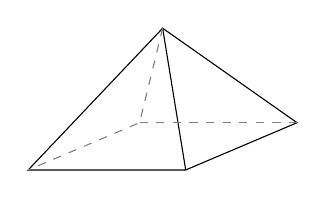
\begin{tikzpicture}[scale=.5, z={(.707,.3)}]
    \draw (2,3,2) -- (0,0,0) -- (4,0,0) -- (4,0,4) -- (2,3,2) 
      -- (4,0,0);
    \draw[color=gray, style=dashed] (2,3,2) -- (0,0,4) 
      -- (0,0,0);
    \draw[color=gray, style=dashed] (0,0,4) -- (4,0,4);
  \end{tikzpicture}

        \label{fig:pyramide}
    }

    \subfloat[$\mdr^2$]{
        \documentclass[varwidth=true, border=2pt]{standalone}
\usepackage{tikz}
\usepackage{tikz-3dplot}

\begin{document}
\tdplotsetmaincoords{110}{50}
\begin{tikzpicture}
		[tdplot_main_coords,
			cube/.style={very thick,black},
			grid/.style={very thin,gray},
			axis/.style={->,blue,thick}]

	%draw a grid in the x-y plane
	\foreach \x in {-0.5,0,...,2.5}
		\foreach \y in {-0.5,0,...,2.5}
		{
			\draw[grid] (\x,-0.5) -- (\x,2.5);
			\draw[grid] (-0.5,\y) -- (2.5,\y);
		}
			

	%draw the axes
	\draw[axis] (-1,0,0) -- (3,0,0) node[anchor=west]{$y$};
	\draw[axis] (0,-1,0) -- (0,3,0) node[anchor=west]{$x$};
	
\end{tikzpicture}
\end{document}

        \label{fig:plane-r2}
    }%
    \subfloat[$T^2$]{
        % Sketch output, version 0.3 (build 7d, Wed May 2 04:54:35 2012)
% Output language: PGF/TikZ,LaTeX
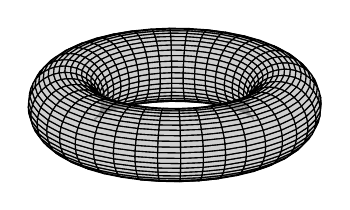
\begin{tikzpicture}[line join=round]
\filldraw[draw=black,fill=lightgray,fill opacity=0.75](-.048,.046)--(-.05,.045)--(.146,.042)--(.138,.044)--cycle;
\filldraw[draw=black,fill=lightgray,fill opacity=0.75](-.232,.038)--(-.246,.036)--(-.05,.045)--(-.048,.046)--cycle;
\filldraw[draw=black,fill=lightgray,fill opacity=0.75](.138,.044)--(.146,.042)--(.339,.028)--(.32,.031)--cycle;
\filldraw[draw=black,fill=lightgray,fill opacity=0.75](-.411,.02)--(-.435,.017)--(-.246,.036)--(-.232,.038)--cycle;
\filldraw[draw=black,fill=lightgray,fill opacity=0.75](.435,.951)--(.417,.954)--(.643,.923)--(.672,.919)--cycle;
\filldraw[draw=black,fill=lightgray,fill opacity=0.75](-.302,.964)--(-.288,.954)--(-.059,.964)--(-.062,.974)--cycle;
\filldraw[draw=black,fill=lightgray,fill opacity=0.75](-.062,.974)--(-.059,.964)--(.171,.961)--(.179,.971)--cycle;
\filldraw[draw=black,fill=lightgray,fill opacity=0.75](.179,.971)--(.171,.961)--(.397,.944)--(.417,.954)--cycle;
\filldraw[draw=black,fill=lightgray,fill opacity=0.75](-.045,.059)--(-.048,.046)--(.138,.044)--(.131,.057)--cycle;
\filldraw[draw=black,fill=lightgray,fill opacity=0.75](-.22,.051)--(-.232,.038)--(-.048,.046)--(-.045,.059)--cycle;
\filldraw[draw=black,fill=lightgray,fill opacity=0.75](-.787,.898)--(-.754,.903)--(-.535,.94)--(-.558,.937)--cycle;
\filldraw[draw=black,fill=lightgray,fill opacity=0.75](.131,.057)--(.138,.044)--(.32,.031)--(.304,.044)--cycle;
\filldraw[draw=black,fill=lightgray,fill opacity=0.75](-.535,.94)--(-.51,.931)--(-.288,.954)--(-.302,.964)--cycle;
\filldraw[draw=black,fill=lightgray,fill opacity=0.75](-.39,.034)--(-.411,.02)--(-.232,.038)--(-.22,.051)--cycle;
\filldraw[draw=black,fill=lightgray,fill opacity=0.75](.417,.954)--(.397,.944)--(.614,.915)--(.643,.923)--cycle;
\filldraw[draw=black,fill=lightgray,fill opacity=0.75](.304,.044)--(.32,.031)--(.495,.007)--(.469,.022)--cycle;
\filldraw[draw=black,fill=lightgray,fill opacity=0.75](.672,.919)--(.643,.923)--(.854,.88)--(.892,.875)--cycle;
\filldraw[draw=black,fill=lightgray,fill opacity=0.75](-.059,.964)--(-.056,.943)--(.163,.94)--(.171,.961)--cycle;
\filldraw[draw=black,fill=lightgray,fill opacity=0.75](-.288,.954)--(-.274,.933)--(-.056,.943)--(-.059,.964)--cycle;
\filldraw[draw=black,fill=lightgray,fill opacity=0.75](.171,.961)--(.163,.94)--(.378,.924)--(.397,.944)--cycle;
\filldraw[draw=black,fill=lightgray,fill opacity=0.75](-.55,.007)--(-.58,-.009)--(-.411,.02)--(-.39,.034)--cycle;
\filldraw[draw=black,fill=lightgray,fill opacity=0.75](-.754,.903)--(-.719,.896)--(-.51,.931)--(-.535,.94)--cycle;
\filldraw[draw=black,fill=lightgray,fill opacity=0.75](-.209,.076)--(-.22,.051)--(-.045,.059)--(-.043,.083)--cycle;
\filldraw[draw=black,fill=lightgray,fill opacity=0.75](-.043,.083)--(-.045,.059)--(.131,.057)--(.124,.081)--cycle;
\filldraw[draw=black,fill=lightgray,fill opacity=0.75](.124,.081)--(.131,.057)--(.304,.044)--(.289,.069)--cycle;
\filldraw[draw=black,fill=lightgray,fill opacity=0.75](-.51,.931)--(-.485,.912)--(-.274,.933)--(-.288,.954)--cycle;
\filldraw[draw=black,fill=lightgray,fill opacity=0.75](-.37,.059)--(-.39,.034)--(-.22,.051)--(-.209,.076)--cycle;
\filldraw[draw=black,fill=lightgray,fill opacity=0.75](.469,.022)--(.495,.007)--(.657,-.026)--(.623,-.009)--cycle;
\filldraw[draw=black,fill=lightgray,fill opacity=0.75](-.997,.847)--(-.955,.853)--(-.754,.903)--(-.787,.898)--cycle;
\filldraw[draw=black,fill=lightgray,fill opacity=0.75](.397,.944)--(.378,.924)--(.583,.897)--(.614,.915)--cycle;
\filldraw[draw=black,fill=lightgray,fill opacity=0.75](.289,.069)--(.304,.044)--(.469,.022)--(.446,.048)--cycle;
\filldraw[draw=black,fill=lightgray,fill opacity=0.75](.643,.923)--(.614,.915)--(.815,.874)--(.854,.88)--cycle;
\filldraw[draw=black,fill=lightgray,fill opacity=0.75](-.056,.943)--(-.053,.911)--(.154,.908)--(.163,.94)--cycle;
\filldraw[draw=black,fill=lightgray,fill opacity=0.75](-.274,.933)--(-.26,.902)--(-.053,.911)--(-.056,.943)--cycle;
\filldraw[draw=black,fill=lightgray,fill opacity=0.75](.163,.94)--(.154,.908)--(.358,.893)--(.378,.924)--cycle;
\filldraw[draw=black,fill=lightgray,fill opacity=0.75](-.522,.033)--(-.55,.007)--(-.39,.034)--(-.37,.059)--cycle;
\filldraw[draw=black,fill=lightgray,fill opacity=0.75](-.719,.896)--(-.684,.878)--(-.485,.912)--(-.51,.931)--cycle;
\filldraw[draw=black,fill=lightgray,fill opacity=0.75](-.696,-.029)--(-.735,-.047)--(-.58,-.009)--(-.55,.007)--cycle;
\filldraw[draw=black,fill=lightgray,fill opacity=0.75](-.2,.11)--(-.209,.076)--(-.043,.083)--(-.041,.117)--cycle;
\filldraw[draw=black,fill=lightgray,fill opacity=0.75](-.041,.117)--(-.043,.083)--(.124,.081)--(.119,.115)--cycle;
\filldraw[draw=black,fill=lightgray,fill opacity=0.75](.119,.115)--(.124,.081)--(.289,.069)--(.276,.104)--cycle;
\filldraw[draw=black,fill=lightgray,fill opacity=0.75](-.485,.912)--(-.459,.881)--(-.26,.902)--(-.274,.933)--cycle;
\filldraw[draw=black,fill=lightgray,fill opacity=0.75](-.354,.095)--(-.37,.059)--(-.209,.076)--(-.2,.11)--cycle;
\filldraw[draw=black,fill=lightgray,fill opacity=0.75](.892,.875)--(.854,.88)--(1.044,.826)--(1.09,.818)--cycle;
\filldraw[draw=black,fill=lightgray,fill opacity=0.75](-.955,.853)--(-.911,.849)--(-.719,.896)--(-.754,.903)--cycle;
\filldraw[draw=black,fill=lightgray,fill opacity=0.75](.446,.048)--(.469,.022)--(.623,-.009)--(.592,.018)--cycle;
\filldraw[draw=black,fill=lightgray,fill opacity=0.75](.378,.924)--(.358,.893)--(.553,.867)--(.583,.897)--cycle;
\filldraw[draw=black,fill=lightgray,fill opacity=0.75](.276,.104)--(.289,.069)--(.446,.048)--(.426,.084)--cycle;
\filldraw[draw=black,fill=lightgray,fill opacity=0.75](.614,.915)--(.583,.897)--(.775,.858)--(.815,.874)--cycle;
\filldraw[draw=black,fill=lightgray,fill opacity=0.75](.623,-.009)--(.657,-.026)--(.804,-.068)--(.761,-.049)--cycle;
\filldraw[draw=black,fill=lightgray,fill opacity=0.75](-.053,.911)--(-.05,.869)--(.146,.866)--(.154,.908)--cycle;
\filldraw[draw=black,fill=lightgray,fill opacity=0.75](-.26,.902)--(-.246,.861)--(-.05,.869)--(-.053,.911)--cycle;
\filldraw[draw=black,fill=lightgray,fill opacity=0.75](.154,.908)--(.146,.866)--(.339,.852)--(.358,.893)--cycle;
\filldraw[draw=black,fill=lightgray,fill opacity=0.75](-.499,.07)--(-.522,.033)--(-.37,.059)--(-.354,.095)--cycle;
\filldraw[draw=black,fill=lightgray,fill opacity=0.75](-.684,.878)--(-.648,.849)--(-.459,.881)--(-.485,.912)--cycle;
\filldraw[draw=black,fill=lightgray,fill opacity=0.75](-.662,-.001)--(-.696,-.029)--(-.55,.007)--(-.522,.033)--cycle;
\filldraw[draw=black,fill=lightgray,fill opacity=0.75](-.04,.161)--(-.041,.117)--(.119,.115)--(.114,.159)--cycle;
\filldraw[draw=black,fill=lightgray,fill opacity=0.75](-.193,.155)--(-.2,.11)--(-.041,.117)--(-.04,.161)--cycle;
\filldraw[draw=black,fill=lightgray,fill opacity=0.75](.114,.159)--(.119,.115)--(.276,.104)--(.265,.148)--cycle;
\filldraw[draw=black,fill=lightgray,fill opacity=0.75](-.459,.881)--(-.435,.841)--(-.246,.861)--(-.26,.902)--cycle;
\filldraw[draw=black,fill=lightgray,fill opacity=0.75](.854,.88)--(.815,.874)--(.996,.822)--(1.044,.826)--cycle;
\filldraw[draw=black,fill=lightgray,fill opacity=0.75](-.341,.139)--(-.354,.095)--(-.2,.11)--(-.193,.155)--cycle;
\filldraw[draw=black,fill=lightgray,fill opacity=0.75](-.911,.849)--(-.866,.833)--(-.684,.878)--(-.719,.896)--cycle;
\filldraw[draw=black,fill=lightgray,fill opacity=0.75](-1.182,.784)--(-1.132,.793)--(-.955,.853)--(-.997,.847)--cycle;
\filldraw[draw=black,fill=lightgray,fill opacity=0.75](.426,.084)--(.446,.048)--(.592,.018)--(.566,.055)--cycle;
\filldraw[draw=black,fill=lightgray,fill opacity=0.75](.358,.893)--(.339,.852)--(.523,.828)--(.553,.867)--cycle;
\filldraw[draw=black,fill=lightgray,fill opacity=0.75](-.825,-.073)--(-.871,-.093)--(-.735,-.047)--(-.696,-.029)--cycle;
\filldraw[draw=black,fill=lightgray,fill opacity=0.75](.265,.148)--(.276,.104)--(.426,.084)--(.41,.129)--cycle;
\filldraw[draw=black,fill=lightgray,fill opacity=0.75](.583,.897)--(.553,.867)--(.734,.83)--(.775,.858)--cycle;
\filldraw[draw=black,fill=lightgray,fill opacity=0.75](.592,.018)--(.623,-.009)--(.761,-.049)--(.724,-.02)--cycle;
\filldraw[draw=black,fill=lightgray,fill opacity=0.75](-.05,.869)--(-.048,.818)--(.138,.816)--(.146,.866)--cycle;
\filldraw[draw=black,fill=lightgray,fill opacity=0.75](-.246,.861)--(-.232,.81)--(-.048,.818)--(-.05,.869)--cycle;
\filldraw[draw=black,fill=lightgray,fill opacity=0.75](.146,.866)--(.138,.816)--(.32,.803)--(.339,.852)--cycle;
\filldraw[draw=black,fill=lightgray,fill opacity=0.75](-.038,.214)--(-.04,.161)--(.114,.159)--(.111,.212)--cycle;
\filldraw[draw=black,fill=lightgray,fill opacity=0.75](-.187,.208)--(-.193,.155)--(-.04,.161)--(-.038,.214)--cycle;
\filldraw[draw=black,fill=lightgray,fill opacity=0.75](-.481,.116)--(-.499,.07)--(-.354,.095)--(-.341,.139)--cycle;
\filldraw[draw=black,fill=lightgray,fill opacity=0.75](-.648,.849)--(-.613,.811)--(-.435,.841)--(-.459,.881)--cycle;
\filldraw[draw=black,fill=lightgray,fill opacity=0.75](-.632,.038)--(-.662,-.001)--(-.522,.033)--(-.499,.07)--cycle;
\filldraw[draw=black,fill=lightgray,fill opacity=0.75](.111,.212)--(.114,.159)--(.265,.148)--(.258,.201)--cycle;
\filldraw[draw=black,fill=lightgray,fill opacity=0.75](-.435,.841)--(-.411,.792)--(-.232,.81)--(-.246,.861)--cycle;
\filldraw[draw=black,fill=lightgray,fill opacity=0.75](-.331,.193)--(-.341,.139)--(-.193,.155)--(-.187,.208)--cycle;
\filldraw[draw=black,fill=lightgray,fill opacity=0.75](.815,.874)--(.775,.858)--(.947,.808)--(.996,.822)--cycle;
\filldraw[draw=black,fill=lightgray,fill opacity=0.75](-.866,.833)--(-.821,.807)--(-.648,.849)--(-.684,.878)--cycle;
\filldraw[draw=black,fill=lightgray,fill opacity=0.75](-1.132,.793)--(-1.08,.792)--(-.911,.849)--(-.955,.853)--cycle;
\filldraw[draw=black,fill=lightgray,fill opacity=0.75](.41,.129)--(.426,.084)--(.566,.055)--(.545,.102)--cycle;
\filldraw[draw=black,fill=lightgray,fill opacity=0.75](.761,-.049)--(.804,-.068)--(.93,-.118)--(.881,-.096)--cycle;
\filldraw[draw=black,fill=lightgray,fill opacity=0.75](.339,.852)--(.32,.803)--(.495,.779)--(.523,.828)--cycle;
\filldraw[draw=black,fill=lightgray,fill opacity=0.75](-.784,-.042)--(-.825,-.073)--(-.696,-.029)--(-.662,-.001)--cycle;
\filldraw[draw=black,fill=lightgray,fill opacity=0.75](.258,.201)--(.265,.148)--(.41,.129)--(.398,.183)--cycle;
\filldraw[draw=black,fill=lightgray,fill opacity=0.75](.553,.867)--(.523,.828)--(.695,.793)--(.734,.83)--cycle;
\filldraw[draw=black,fill=lightgray,fill opacity=0.75](-.048,.818)--(-.045,.76)--(.131,.758)--(.138,.816)--cycle;
\filldraw[draw=black,fill=lightgray,fill opacity=0.75](-.232,.81)--(-.22,.753)--(-.045,.76)--(-.048,.818)--cycle;
\filldraw[draw=black,fill=lightgray,fill opacity=0.75](1.09,.818)--(1.044,.826)--(1.209,.761)--(1.262,.75)--cycle;
\filldraw[draw=black,fill=lightgray,fill opacity=0.75](.566,.055)--(.592,.018)--(.724,-.02)--(.691,.019)--cycle;
\filldraw[draw=black,fill=lightgray,fill opacity=0.75](.138,.816)--(.131,.758)--(.304,.745)--(.32,.803)--cycle;
\filldraw[draw=black,fill=lightgray,fill opacity=0.75](-.038,.274)--(-.038,.214)--(.111,.212)--(.109,.272)--cycle;
\filldraw[draw=black,fill=lightgray,fill opacity=0.75](-.184,.268)--(-.187,.208)--(-.038,.214)--(-.038,.274)--cycle;
\filldraw[draw=black,fill=lightgray,fill opacity=0.75](.109,.272)--(.111,.212)--(.258,.201)--(.253,.261)--cycle;
\filldraw[draw=black,fill=lightgray,fill opacity=0.75](-.467,.17)--(-.481,.116)--(-.341,.139)--(-.331,.193)--cycle;
\filldraw[draw=black,fill=lightgray,fill opacity=0.75](-.613,.811)--(-.58,.763)--(-.411,.792)--(-.435,.841)--cycle;
\filldraw[draw=black,fill=lightgray,fill opacity=0.75](-.411,.792)--(-.39,.735)--(-.22,.753)--(-.232,.81)--cycle;
\filldraw[draw=black,fill=lightgray,fill opacity=0.75](-.609,.085)--(-.632,.038)--(-.499,.07)--(-.481,.116)--cycle;
\filldraw[draw=black,fill=lightgray,fill opacity=0.75](-.325,.253)--(-.331,.193)--(-.187,.208)--(-.184,.268)--cycle;
\filldraw[draw=black,fill=lightgray,fill opacity=0.75](-1.39,.689)--(-1.338,.712)--(-1.182,.784)--(-1.228,.764)--cycle;
\filldraw[draw=black,fill=lightgray,fill opacity=0.75](.775,.858)--(.734,.83)--(.897,.783)--(.947,.808)--cycle;
\filldraw[draw=black,fill=lightgray,fill opacity=0.75](.32,.803)--(.304,.745)--(.469,.723)--(.495,.779)--cycle;
\filldraw[draw=black,fill=lightgray,fill opacity=0.75](.398,.183)--(.41,.129)--(.545,.102)--(.529,.156)--cycle;
\filldraw[draw=black,fill=lightgray,fill opacity=0.75](.253,.261)--(.258,.201)--(.398,.183)--(.391,.243)--cycle;
\filldraw[draw=black,fill=lightgray,fill opacity=0.75](-.045,.76)--(-.043,.696)--(.124,.693)--(.131,.758)--cycle;
\filldraw[draw=black,fill=lightgray,fill opacity=0.75](-.22,.753)--(-.209,.689)--(-.043,.696)--(-.045,.76)--cycle;
\filldraw[draw=black,fill=lightgray,fill opacity=0.75](-.821,.807)--(-.776,.771)--(-.613,.811)--(-.648,.849)--cycle;
\filldraw[draw=black,fill=lightgray,fill opacity=0.75](.724,-.02)--(.761,-.049)--(.881,-.096)--(.837,-.065)--cycle;
\filldraw[draw=black,fill=lightgray,fill opacity=0.75](-1.08,.792)--(-1.026,.779)--(-.866,.833)--(-.911,.849)--cycle;
\filldraw[draw=black,fill=lightgray,fill opacity=0.75](.131,.758)--(.124,.693)--(.289,.682)--(.304,.745)--cycle;
\filldraw[draw=black,fill=lightgray,fill opacity=0.75](-.75,-.002)--(-.784,-.042)--(-.662,-.001)--(-.632,.038)--cycle;
\filldraw[draw=black,fill=lightgray,fill opacity=0.75](-.038,.34)--(-.038,.274)--(.109,.272)--(.108,.338)--cycle;
\filldraw[draw=black,fill=lightgray,fill opacity=0.75](-.183,.333)--(-.184,.268)--(-.038,.274)--(-.038,.34)--cycle;
\filldraw[draw=black,fill=lightgray,fill opacity=0.75](.523,.828)--(.495,.779)--(.657,.746)--(.695,.793)--cycle;
\filldraw[draw=black,fill=lightgray,fill opacity=0.75](.108,.338)--(.109,.272)--(.253,.261)--(.252,.327)--cycle;
\filldraw[draw=black,fill=lightgray,fill opacity=0.75](1.044,.826)--(.996,.822)--(1.153,.761)--(1.209,.761)--cycle;
\filldraw[draw=black,fill=lightgray,fill opacity=0.75](.545,.102)--(.566,.055)--(.691,.019)--(.666,.067)--cycle;
\filldraw[draw=black,fill=lightgray,fill opacity=0.75](-.39,.735)--(-.37,.672)--(-.209,.689)--(-.22,.753)--cycle;
\filldraw[draw=black,fill=lightgray,fill opacity=0.75](-.459,.23)--(-.467,.17)--(-.331,.193)--(-.325,.253)--cycle;
\filldraw[draw=black,fill=lightgray,fill opacity=0.75](-.58,.763)--(-.55,.708)--(-.39,.735)--(-.411,.792)--cycle;
\filldraw[draw=black,fill=lightgray,fill opacity=0.75](-.323,.319)--(-.325,.253)--(-.184,.268)--(-.183,.333)--cycle;
\filldraw[draw=black,fill=lightgray,fill opacity=0.75](-.591,.139)--(-.609,.085)--(-.481,.116)--(-.467,.17)--cycle;
\filldraw[draw=black,fill=lightgray,fill opacity=0.75](-.209,.689)--(-.2,.62)--(-.041,.627)--(-.043,.696)--cycle;
\filldraw[draw=black,fill=lightgray,fill opacity=0.75](-.043,.696)--(-.041,.627)--(.119,.625)--(.124,.693)--cycle;
\filldraw[draw=black,fill=lightgray,fill opacity=0.75](.304,.745)--(.289,.682)--(.446,.661)--(.469,.723)--cycle;
\filldraw[draw=black,fill=lightgray,fill opacity=0.75](.124,.693)--(.119,.625)--(.276,.613)--(.289,.682)--cycle;
\filldraw[draw=black,fill=lightgray,fill opacity=0.75](.252,.327)--(.253,.261)--(.391,.243)--(.389,.309)--cycle;
\filldraw[draw=black,fill=lightgray,fill opacity=0.75](-.038,.41)--(-.038,.34)--(.108,.338)--(.109,.407)--cycle;
\filldraw[draw=black,fill=lightgray,fill opacity=0.75](-.184,.403)--(-.183,.333)--(-.038,.34)--(-.038,.41)--cycle;
\filldraw[draw=black,fill=lightgray,fill opacity=0.75](-1.338,.712)--(-1.282,.724)--(-1.132,.793)--(-1.182,.784)--cycle;
\filldraw[draw=black,fill=lightgray,fill opacity=0.75](.109,.407)--(.108,.338)--(.252,.327)--(.253,.397)--cycle;
\filldraw[draw=black,fill=lightgray,fill opacity=0.75](.391,.243)--(.398,.183)--(.529,.156)--(.52,.217)--cycle;
\filldraw[draw=black,fill=lightgray,fill opacity=0.75](.734,.83)--(.695,.793)--(.849,.748)--(.897,.783)--cycle;
\filldraw[draw=black,fill=lightgray,fill opacity=0.75](-.776,.771)--(-.735,.726)--(-.58,.763)--(-.613,.811)--cycle;
\filldraw[draw=black,fill=lightgray,fill opacity=0.75](-.37,.672)--(-.354,.604)--(-.2,.62)--(-.209,.689)--cycle;
\filldraw[draw=black,fill=lightgray,fill opacity=0.75](.495,.779)--(.469,.723)--(.623,.692)--(.657,.746)--cycle;
\filldraw[draw=black,fill=lightgray,fill opacity=0.75](.691,.019)--(.724,-.02)--(.837,-.065)--(.8,-.024)--cycle;
\filldraw[draw=black,fill=lightgray,fill opacity=0.75](-1.026,.779)--(-.973,.756)--(-.821,.807)--(-.866,.833)--cycle;
\filldraw[draw=black,fill=lightgray,fill opacity=0.75](-.325,.389)--(-.323,.319)--(-.183,.333)--(-.184,.403)--cycle;
\filldraw[draw=black,fill=lightgray,fill opacity=0.75](-.2,.62)--(-.193,.548)--(-.04,.555)--(-.041,.627)--cycle;
\filldraw[draw=black,fill=lightgray,fill opacity=0.75](-.041,.627)--(-.04,.555)--(.114,.553)--(.119,.625)--cycle;
\filldraw[draw=black,fill=lightgray,fill opacity=0.75](-.888,-.09)--(-.934,-.123)--(-.825,-.073)--(-.784,-.042)--cycle;
\filldraw[draw=black,fill=lightgray,fill opacity=0.75](-.722,.046)--(-.75,-.002)--(-.632,.038)--(-.609,.085)--cycle;
\filldraw[draw=black,fill=lightgray,fill opacity=0.75](-.038,.482)--(-.038,.41)--(.109,.407)--(.111,.48)--cycle;
\filldraw[draw=black,fill=lightgray,fill opacity=0.75](-.187,.475)--(-.184,.403)--(-.038,.41)--(-.038,.482)--cycle;
\filldraw[draw=black,fill=lightgray,fill opacity=0.75](-.456,.296)--(-.459,.23)--(-.325,.253)--(-.323,.319)--cycle;
\filldraw[draw=black,fill=lightgray,fill opacity=0.75](.119,.625)--(.114,.553)--(.265,.542)--(.276,.613)--cycle;
\filldraw[draw=black,fill=lightgray,fill opacity=0.75](-.55,.708)--(-.522,.646)--(-.37,.672)--(-.39,.735)--cycle;
\filldraw[draw=black,fill=lightgray,fill opacity=0.75](.111,.48)--(.109,.407)--(.253,.397)--(.258,.469)--cycle;
\filldraw[draw=black,fill=lightgray,fill opacity=0.75](.529,.156)--(.545,.102)--(.666,.067)--(.647,.122)--cycle;
\filldraw[draw=black,fill=lightgray,fill opacity=0.75](.996,.822)--(.947,.808)--(1.096,.749)--(1.153,.761)--cycle;
\filldraw[draw=black,fill=lightgray,fill opacity=0.75](.289,.682)--(.276,.613)--(.426,.593)--(.446,.661)--cycle;
\filldraw[draw=black,fill=lightgray,fill opacity=0.75](-.04,.555)--(-.038,.482)--(.111,.48)--(.114,.553)--cycle;
\filldraw[draw=black,fill=lightgray,fill opacity=0.75](-.193,.548)--(-.187,.475)--(-.038,.482)--(-.04,.555)--cycle;
\filldraw[draw=black,fill=lightgray,fill opacity=0.75](.253,.397)--(.252,.327)--(.389,.309)--(.391,.379)--cycle;
\filldraw[draw=black,fill=lightgray,fill opacity=0.75](-.354,.604)--(-.341,.533)--(-.193,.548)--(-.2,.62)--cycle;
\filldraw[draw=black,fill=lightgray,fill opacity=0.75](.114,.553)--(.111,.48)--(.258,.469)--(.265,.542)--cycle;
\filldraw[draw=black,fill=lightgray,fill opacity=0.75](-.331,.461)--(-.325,.389)--(-.184,.403)--(-.187,.475)--cycle;
\filldraw[draw=black,fill=lightgray,fill opacity=0.75](-.581,.201)--(-.591,.139)--(-.467,.17)--(-.459,.23)--cycle;
\filldraw[draw=black,fill=lightgray,fill opacity=0.75](1.31,.729)--(1.262,.75)--(1.402,.673)--(1.456,.649)--cycle;
\filldraw[draw=black,fill=lightgray,fill opacity=0.75](-.341,.533)--(-.331,.461)--(-.187,.475)--(-.193,.548)--cycle;
\filldraw[draw=black,fill=lightgray,fill opacity=0.75](.389,.309)--(.391,.243)--(.52,.217)--(.516,.283)--cycle;
\filldraw[draw=black,fill=lightgray,fill opacity=0.75](.276,.613)--(.265,.542)--(.41,.522)--(.426,.593)--cycle;
\filldraw[draw=black,fill=lightgray,fill opacity=0.75](.258,.469)--(.253,.397)--(.391,.379)--(.398,.45)--cycle;
\filldraw[draw=black,fill=lightgray,fill opacity=0.75](-.459,.366)--(-.456,.296)--(-.323,.319)--(-.325,.389)--cycle;
\filldraw[draw=black,fill=lightgray,fill opacity=0.75](.469,.723)--(.446,.661)--(.592,.631)--(.623,.692)--cycle;
\filldraw[draw=black,fill=lightgray,fill opacity=0.75](-.522,.646)--(-.499,.579)--(-.354,.604)--(-.37,.672)--cycle;
\filldraw[draw=black,fill=lightgray,fill opacity=0.75](-.735,.726)--(-.696,.672)--(-.55,.708)--(-.58,.763)--cycle;
\filldraw[draw=black,fill=lightgray,fill opacity=0.75](-1.282,.724)--(-1.222,.726)--(-1.08,.792)--(-1.132,.793)--cycle;
\filldraw[draw=black,fill=lightgray,fill opacity=0.75](.695,.793)--(.657,.746)--(.804,.704)--(.849,.748)--cycle;
\filldraw[draw=black,fill=lightgray,fill opacity=0.75](.265,.542)--(.258,.469)--(.398,.45)--(.41,.522)--cycle;
\filldraw[draw=black,fill=lightgray,fill opacity=0.75](-.973,.756)--(-.921,.722)--(-.776,.771)--(-.821,.807)--cycle;
\filldraw[draw=black,fill=lightgray,fill opacity=0.75](.666,.067)--(.691,.019)--(.8,-.024)--(.77,.025)--cycle;
\filldraw[draw=black,fill=lightgray,fill opacity=0.75](-.701,.102)--(-.722,.046)--(-.609,.085)--(-.591,.139)--cycle;
\filldraw[draw=black,fill=lightgray,fill opacity=0.75](-.849,-.048)--(-.888,-.09)--(-.784,-.042)--(-.75,-.002)--cycle;
\filldraw[draw=black,fill=lightgray,fill opacity=0.75](.52,.217)--(.529,.156)--(.647,.122)--(.635,.184)--cycle;
\filldraw[draw=black,fill=lightgray,fill opacity=0.75](-.467,.438)--(-.459,.366)--(-.325,.389)--(-.331,.461)--cycle;
\filldraw[draw=black,fill=lightgray,fill opacity=0.75](-.499,.579)--(-.481,.509)--(-.341,.533)--(-.354,.604)--cycle;
\filldraw[draw=black,fill=lightgray,fill opacity=0.75](.391,.379)--(.389,.309)--(.516,.283)--(.52,.352)--cycle;
\filldraw[draw=black,fill=lightgray,fill opacity=0.75](-.577,.267)--(-.581,.201)--(-.459,.23)--(-.456,.296)--cycle;
\filldraw[draw=black,fill=lightgray,fill opacity=0.75](.947,.808)--(.897,.783)--(1.039,.728)--(1.096,.749)--cycle;
\filldraw[draw=black,fill=lightgray,fill opacity=0.75](.837,-.065)--(.881,-.096)--(.979,-.15)--(.931,-.116)--cycle;
\filldraw[draw=black,fill=lightgray,fill opacity=0.75](.446,.661)--(.426,.593)--(.566,.565)--(.592,.631)--cycle;
\filldraw[draw=black,fill=lightgray,fill opacity=0.75](-.481,.509)--(-.467,.438)--(-.331,.461)--(-.341,.533)--cycle;
\filldraw[draw=black,fill=lightgray,fill opacity=0.75](1.262,.75)--(1.209,.761)--(1.343,.687)--(1.402,.673)--cycle;
\filldraw[draw=black,fill=lightgray,fill opacity=0.75](-.696,.672)--(-.662,.612)--(-.522,.646)--(-.55,.708)--cycle;
\filldraw[draw=black,fill=lightgray,fill opacity=0.75](.657,.746)--(.623,.692)--(.761,.652)--(.804,.704)--cycle;
\filldraw[draw=black,fill=lightgray,fill opacity=0.75](.398,.45)--(.391,.379)--(.52,.352)--(.529,.424)--cycle;
\filldraw[draw=black,fill=lightgray,fill opacity=0.75](.426,.593)--(.41,.522)--(.545,.495)--(.566,.565)--cycle;
\filldraw[draw=black,fill=lightgray,fill opacity=0.75](-1.222,.726)--(-1.162,.716)--(-1.026,.779)--(-1.08,.792)--cycle;
\filldraw[draw=black,fill=lightgray,fill opacity=0.75](-.581,.336)--(-.577,.267)--(-.456,.296)--(-.459,.366)--cycle;
\filldraw[draw=black,fill=lightgray,fill opacity=0.75](.41,.522)--(.398,.45)--(.529,.424)--(.545,.495)--cycle;
\filldraw[draw=black,fill=lightgray,fill opacity=0.75](-.921,.722)--(-.871,.68)--(-.735,.726)--(-.776,.771)--cycle;
\filldraw[draw=black,fill=lightgray,fill opacity=0.75](.516,.283)--(.52,.217)--(.635,.184)--(.631,.25)--cycle;
\filldraw[draw=black,fill=lightgray,fill opacity=0.75](-.688,.164)--(-.701,.102)--(-.591,.139)--(-.581,.201)--cycle;
\filldraw[draw=black,fill=lightgray,fill opacity=0.75](.647,.122)--(.666,.067)--(.77,.025)--(.748,.082)--cycle;
\filldraw[draw=black,fill=lightgray,fill opacity=0.75](-.662,.612)--(-.632,.547)--(-.499,.579)--(-.522,.646)--cycle;
\filldraw[draw=black,fill=lightgray,fill opacity=0.75](-.817,.002)--(-.849,-.048)--(-.75,-.002)--(-.722,.046)--cycle;
\filldraw[draw=black,fill=lightgray,fill opacity=0.75](.897,.783)--(.849,.748)--(.983,.696)--(1.039,.728)--cycle;
\filldraw[draw=black,fill=lightgray,fill opacity=0.75](.8,-.024)--(.837,-.065)--(.931,-.116)--(.889,-.072)--cycle;
\filldraw[draw=black,fill=lightgray,fill opacity=0.75](-.591,.407)--(-.581,.336)--(-.459,.366)--(-.467,.438)--cycle;
\filldraw[draw=black,fill=lightgray,fill opacity=0.75](.623,.692)--(.592,.631)--(.724,.593)--(.761,.652)--cycle;
\filldraw[draw=black,fill=lightgray,fill opacity=0.75](-.632,.547)--(-.609,.478)--(-.481,.509)--(-.499,.579)--cycle;
\filldraw[draw=black,fill=lightgray,fill opacity=0.75](1.209,.761)--(1.153,.761)--(1.281,.691)--(1.343,.687)--cycle;
\filldraw[draw=black,fill=lightgray,fill opacity=0.75](-1.517,.605)--(-1.461,.631)--(-1.338,.712)--(-1.39,.689)--cycle;
\filldraw[draw=black,fill=lightgray,fill opacity=0.75](-.609,.478)--(-.591,.407)--(-.467,.438)--(-.481,.509)--cycle;
\filldraw[draw=black,fill=lightgray,fill opacity=0.75](.52,.352)--(.516,.283)--(.631,.25)--(.635,.319)--cycle;
\filldraw[draw=black,fill=lightgray,fill opacity=0.75](-.97,-.144)--(-1.02,-.179)--(-.934,-.123)--(-.888,-.09)--cycle;
\filldraw[draw=black,fill=lightgray,fill opacity=0.75](-.871,.68)--(-.825,.629)--(-.696,.672)--(-.735,.726)--cycle;
\filldraw[draw=black,fill=lightgray,fill opacity=0.75](-1.162,.716)--(-1.101,.696)--(-.973,.756)--(-1.026,.779)--cycle;
\filldraw[draw=black,fill=lightgray,fill opacity=0.75](-.684,.23)--(-.688,.164)--(-.581,.201)--(-.577,.267)--cycle;
\filldraw[draw=black,fill=lightgray,fill opacity=0.75](.592,.631)--(.566,.565)--(.691,.528)--(.724,.593)--cycle;
\filldraw[draw=black,fill=lightgray,fill opacity=0.75](.635,.184)--(.647,.122)--(.748,.082)--(.735,.144)--cycle;
\filldraw[draw=black,fill=lightgray,fill opacity=0.75](.529,.424)--(.52,.352)--(.635,.319)--(.647,.39)--cycle;
\filldraw[draw=black,fill=lightgray,fill opacity=0.75](-.794,.059)--(-.817,.002)--(-.722,.046)--(-.701,.102)--cycle;
\filldraw[draw=black,fill=lightgray,fill opacity=0.75](.849,.748)--(.804,.704)--(.93,.654)--(.983,.696)--cycle;
\filldraw[draw=black,fill=lightgray,fill opacity=0.75](.566,.565)--(.545,.495)--(.666,.46)--(.691,.528)--cycle;
\filldraw[draw=black,fill=lightgray,fill opacity=0.75](.77,.025)--(.8,-.024)--(.889,-.072)--(.856,-.021)--cycle;
\filldraw[draw=black,fill=lightgray,fill opacity=0.75](.545,.495)--(.529,.424)--(.647,.39)--(.666,.46)--cycle;
\filldraw[draw=black,fill=lightgray,fill opacity=0.75](-.825,.629)--(-.784,.571)--(-.662,.612)--(-.696,.672)--cycle;
\filldraw[draw=black,fill=lightgray,fill opacity=0.75](-.688,.3)--(-.684,.23)--(-.577,.267)--(-.581,.336)--cycle;
\filldraw[draw=black,fill=lightgray,fill opacity=0.75](1.153,.761)--(1.096,.749)--(1.218,.683)--(1.281,.691)--cycle;
\filldraw[draw=black,fill=lightgray,fill opacity=0.75](-1.461,.631)--(-1.399,.647)--(-1.282,.724)--(-1.338,.712)--cycle;
\filldraw[draw=black,fill=lightgray,fill opacity=0.75](-.927,-.099)--(-.97,-.144)--(-.888,-.09)--(-.849,-.048)--cycle;
\filldraw[draw=black,fill=lightgray,fill opacity=0.75](-1.101,.696)--(-1.042,.666)--(-.921,.722)--(-.973,.756)--cycle;
\filldraw[draw=black,fill=lightgray,fill opacity=0.75](.631,.25)--(.635,.184)--(.735,.144)--(.73,.211)--cycle;
\filldraw[draw=black,fill=lightgray,fill opacity=0.75](1.505,.615)--(1.456,.649)--(1.566,.562)--(1.618,.525)--cycle;
\filldraw[draw=black,fill=lightgray,fill opacity=0.75](.804,.704)--(.761,.652)--(.881,.605)--(.93,.654)--cycle;
\filldraw[draw=black,fill=lightgray,fill opacity=0.75](-.784,.571)--(-.75,.507)--(-.632,.547)--(-.662,.612)--cycle;
\filldraw[draw=black,fill=lightgray,fill opacity=0.75](-.701,.37)--(-.688,.3)--(-.581,.336)--(-.591,.407)--cycle;
\filldraw[draw=black,fill=lightgray,fill opacity=0.75](-.779,.122)--(-.794,.059)--(-.701,.102)--(-.688,.164)--cycle;
\filldraw[draw=black,fill=lightgray,fill opacity=0.75](-.75,.507)--(-.722,.44)--(-.609,.478)--(-.632,.547)--cycle;
\filldraw[draw=black,fill=lightgray,fill opacity=0.75](-.722,.44)--(-.701,.37)--(-.591,.407)--(-.609,.478)--cycle;
\filldraw[draw=black,fill=lightgray,fill opacity=0.75](.748,.082)--(.77,.025)--(.856,-.021)--(.832,.037)--cycle;
\filldraw[draw=black,fill=lightgray,fill opacity=0.75](.635,.319)--(.631,.25)--(.73,.211)--(.735,.28)--cycle;
\filldraw[draw=black,fill=lightgray,fill opacity=0.75](1.096,.749)--(1.039,.728)--(1.154,.665)--(1.218,.683)--cycle;
\filldraw[draw=black,fill=lightgray,fill opacity=0.75](-1.399,.647)--(-1.335,.652)--(-1.222,.726)--(-1.282,.724)--cycle;
\filldraw[draw=black,fill=lightgray,fill opacity=0.75](.761,.652)--(.724,.593)--(.837,.548)--(.881,.605)--cycle;
\filldraw[draw=black,fill=lightgray,fill opacity=0.75](-1.042,.666)--(-.986,.626)--(-.871,.68)--(-.921,.722)--cycle;
\filldraw[draw=black,fill=lightgray,fill opacity=0.75](-.892,-.047)--(-.927,-.099)--(-.849,-.048)--(-.817,.002)--cycle;
\filldraw[draw=black,fill=lightgray,fill opacity=0.75](1.456,.649)--(1.402,.673)--(1.508,.59)--(1.566,.562)--cycle;
\filldraw[draw=black,fill=lightgray,fill opacity=0.75](-.775,.189)--(-.779,.122)--(-.688,.164)--(-.684,.23)--cycle;
\filldraw[draw=black,fill=lightgray,fill opacity=0.75](.647,.39)--(.635,.319)--(.735,.28)--(.748,.35)--cycle;
\filldraw[draw=black,fill=lightgray,fill opacity=0.75](.724,.593)--(.691,.528)--(.8,.486)--(.837,.548)--cycle;
\filldraw[draw=black,fill=lightgray,fill opacity=0.75](.889,-.072)--(.931,-.116)--(1.001,-.171)--(.956,-.125)--cycle;
\filldraw[draw=black,fill=lightgray,fill opacity=0.75](.735,.144)--(.748,.082)--(.832,.037)--(.817,.1)--cycle;
\filldraw[draw=black,fill=lightgray,fill opacity=0.75](.666,.46)--(.647,.39)--(.748,.35)--(.77,.419)--cycle;
\filldraw[draw=black,fill=lightgray,fill opacity=0.75](.691,.528)--(.666,.46)--(.77,.419)--(.8,.486)--cycle;
\filldraw[draw=black,fill=lightgray,fill opacity=0.75](-.986,.626)--(-.934,.578)--(-.825,.629)--(-.871,.68)--cycle;
\filldraw[draw=black,fill=lightgray,fill opacity=0.75](1.039,.728)--(.983,.696)--(1.092,.636)--(1.154,.665)--cycle;
\filldraw[draw=black,fill=lightgray,fill opacity=0.75](-1.335,.652)--(-1.269,.646)--(-1.162,.716)--(-1.222,.726)--cycle;
\filldraw[draw=black,fill=lightgray,fill opacity=0.75](-.779,.258)--(-.775,.189)--(-.684,.23)--(-.688,.3)--cycle;
\filldraw[draw=black,fill=lightgray,fill opacity=0.75](-.867,.012)--(-.892,-.047)--(-.817,.002)--(-.794,.059)--cycle;
\filldraw[draw=black,fill=lightgray,fill opacity=0.75](1.402,.673)--(1.343,.687)--(1.445,.607)--(1.508,.59)--cycle;
\filldraw[draw=black,fill=lightgray,fill opacity=0.75](-.934,.578)--(-.888,.523)--(-.784,.571)--(-.825,.629)--cycle;
\filldraw[draw=black,fill=lightgray,fill opacity=0.75](.73,.211)--(.735,.144)--(.817,.1)--(.812,.166)--cycle;
\filldraw[draw=black,fill=lightgray,fill opacity=0.75](.856,-.021)--(.889,-.072)--(.956,-.125)--(.921,-.072)--cycle;
\filldraw[draw=black,fill=lightgray,fill opacity=0.75](-.794,.327)--(-.779,.258)--(-.688,.3)--(-.701,.37)--cycle;
\filldraw[draw=black,fill=lightgray,fill opacity=0.75](.983,.696)--(.93,.654)--(1.033,.598)--(1.092,.636)--cycle;
\filldraw[draw=black,fill=lightgray,fill opacity=0.75](-.888,.523)--(-.849,.461)--(-.75,.507)--(-.784,.571)--cycle;
\filldraw[draw=black,fill=lightgray,fill opacity=0.75](-1.269,.646)--(-1.203,.63)--(-1.101,.696)--(-1.162,.716)--cycle;
\filldraw[draw=black,fill=lightgray,fill opacity=0.75](-1.661,.477)--(-1.608,.515)--(-1.517,.605)--(-1.568,.57)--cycle;
\filldraw[draw=black,fill=lightgray,fill opacity=0.75](-.817,.396)--(-.794,.327)--(-.701,.37)--(-.722,.44)--cycle;
\filldraw[draw=black,fill=lightgray,fill opacity=0.75](-.851,.075)--(-.867,.012)--(-.794,.059)--(-.779,.122)--cycle;
\filldraw[draw=black,fill=lightgray,fill opacity=0.75](-.849,.461)--(-.817,.396)--(-.722,.44)--(-.75,.507)--cycle;
\filldraw[draw=black,fill=lightgray,fill opacity=0.75](1.343,.687)--(1.281,.691)--(1.378,.614)--(1.445,.607)--cycle;
\filldraw[draw=black,fill=lightgray,fill opacity=0.75](.735,.28)--(.73,.211)--(.812,.166)--(.817,.235)--cycle;
\filldraw[draw=black,fill=lightgray,fill opacity=0.75](-.982,-.154)--(-1.028,-.201)--(-.97,-.144)--(-.927,-.099)--cycle;
\filldraw[draw=black,fill=lightgray,fill opacity=0.75](.93,.654)--(.881,.605)--(.979,.551)--(1.033,.598)--cycle;
\filldraw[draw=black,fill=lightgray,fill opacity=0.75](.832,.037)--(.856,-.021)--(.921,-.072)--(.894,-.013)--cycle;
\filldraw[draw=black,fill=lightgray,fill opacity=0.75](-1.203,.63)--(-1.138,.603)--(-1.042,.666)--(-1.101,.696)--cycle;
\filldraw[draw=black,fill=lightgray,fill opacity=0.75](.748,.35)--(.735,.28)--(.817,.235)--(.832,.304)--cycle;
\filldraw[draw=black,fill=lightgray,fill opacity=0.75](-1.608,.515)--(-1.548,.545)--(-1.461,.631)--(-1.517,.605)--cycle;
\filldraw[draw=black,fill=lightgray,fill opacity=0.75](.881,.605)--(.837,.548)--(.931,.497)--(.979,.551)--cycle;
\filldraw[draw=black,fill=lightgray,fill opacity=0.75](-.846,.142)--(-.851,.075)--(-.779,.122)--(-.775,.189)--cycle;
\filldraw[draw=black,fill=lightgray,fill opacity=0.75](1.281,.691)--(1.218,.683)--(1.31,.61)--(1.378,.614)--cycle;
\filldraw[draw=black,fill=lightgray,fill opacity=0.75](.77,.419)--(.748,.35)--(.832,.304)--(.856,.372)--cycle;
\filldraw[draw=black,fill=lightgray,fill opacity=0.75](-.945,-.1)--(-.982,-.154)--(-.927,-.099)--(-.892,-.047)--cycle;
\filldraw[draw=black,fill=lightgray,fill opacity=0.75](.837,.548)--(.8,.486)--(.889,.437)--(.931,.497)--cycle;
\filldraw[draw=black,fill=lightgray,fill opacity=0.75](.8,.486)--(.77,.419)--(.856,.372)--(.889,.437)--cycle;
\filldraw[draw=black,fill=lightgray,fill opacity=0.75](.817,.1)--(.832,.037)--(.894,-.013)--(.878,.051)--cycle;
\filldraw[draw=black,fill=lightgray,fill opacity=0.75](-1.138,.603)--(-1.077,.567)--(-.986,.626)--(-1.042,.666)--cycle;
\filldraw[draw=black,fill=lightgray,fill opacity=0.75](-.851,.211)--(-.846,.142)--(-.775,.189)--(-.779,.258)--cycle;
\filldraw[draw=black,fill=lightgray,fill opacity=0.75](-1.548,.545)--(-1.483,.564)--(-1.399,.647)--(-1.461,.631)--cycle;
\filldraw[draw=black,fill=lightgray,fill opacity=0.75](1.663,.479)--(1.618,.525)--(1.692,.43)--(1.739,.382)--cycle;
\filldraw[draw=black,fill=lightgray,fill opacity=0.75](1.218,.683)--(1.154,.665)--(1.241,.596)--(1.31,.61)--cycle;
\filldraw[draw=black,fill=lightgray,fill opacity=0.75](-1.077,.567)--(-1.02,.522)--(-.934,.578)--(-.986,.626)--cycle;
\filldraw[draw=black,fill=lightgray,fill opacity=0.75](-.918,-.04)--(-.945,-.1)--(-.892,-.047)--(-.867,.012)--cycle;
\filldraw[draw=black,fill=lightgray,fill opacity=0.75](-.867,.279)--(-.851,.211)--(-.779,.258)--(-.794,.327)--cycle;
\filldraw[draw=black,fill=lightgray,fill opacity=0.75](.812,.166)--(.817,.1)--(.878,.051)--(.873,.118)--cycle;
\filldraw[draw=black,fill=lightgray,fill opacity=0.75](-1.02,.522)--(-.97,.469)--(-.888,.523)--(-.934,.578)--cycle;
\filldraw[draw=black,fill=lightgray,fill opacity=0.75](-.892,.346)--(-.867,.279)--(-.794,.327)--(-.817,.396)--cycle;
\filldraw[draw=black,fill=lightgray,fill opacity=0.75](1.618,.525)--(1.566,.562)--(1.638,.47)--(1.692,.43)--cycle;
\filldraw[draw=black,fill=lightgray,fill opacity=0.75](-1.483,.564)--(-1.414,.573)--(-1.335,.652)--(-1.399,.647)--cycle;
\filldraw[draw=black,fill=lightgray,fill opacity=0.75](1.154,.665)--(1.092,.636)--(1.175,.571)--(1.241,.596)--cycle;
\filldraw[draw=black,fill=lightgray,fill opacity=0.75](-.97,.469)--(-.927,.41)--(-.849,.461)--(-.888,.523)--cycle;
\filldraw[draw=black,fill=lightgray,fill opacity=0.75](-.927,.41)--(-.892,.346)--(-.817,.396)--(-.849,.461)--cycle;
\filldraw[draw=black,fill=lightgray,fill opacity=0.75](.921,-.072)--(.956,-.125)--(1,-.182)--(.963,-.126)--cycle;
\filldraw[draw=black,fill=lightgray,fill opacity=0.75](.817,.235)--(.812,.166)--(.873,.118)--(.878,.187)--cycle;
\filldraw[draw=black,fill=lightgray,fill opacity=0.75](-.902,.025)--(-.918,-.04)--(-.867,.012)--(-.851,.075)--cycle;
\filldraw[draw=black,fill=lightgray,fill opacity=0.75](1.092,.636)--(1.033,.598)--(1.111,.536)--(1.175,.571)--cycle;
\filldraw[draw=black,fill=lightgray,fill opacity=0.75](-1.414,.573)--(-1.344,.571)--(-1.269,.646)--(-1.335,.652)--cycle;
\filldraw[draw=black,fill=lightgray,fill opacity=0.75](1.566,.562)--(1.508,.59)--(1.577,.501)--(1.638,.47)--cycle;
\filldraw[draw=black,fill=lightgray,fill opacity=0.75](.832,.304)--(.817,.235)--(.878,.187)--(.894,.255)--cycle;
\filldraw[draw=black,fill=lightgray,fill opacity=0.75](.894,-.013)--(.921,-.072)--(.963,-.126)--(.935,-.066)--cycle;
\filldraw[draw=black,fill=lightgray,fill opacity=0.75](-.896,.092)--(-.902,.025)--(-.851,.075)--(-.846,.142)--cycle;
\filldraw[draw=black,fill=lightgray,fill opacity=0.75](1.033,.598)--(.979,.551)--(1.053,.493)--(1.111,.536)--cycle;
\filldraw[draw=black,fill=lightgray,fill opacity=0.75](.856,.372)--(.832,.304)--(.894,.255)--(.921,.321)--cycle;
\filldraw[draw=black,fill=lightgray,fill opacity=0.75](-1.799,.274)--(-1.761,.33)--(-1.707,.43)--(-1.744,.376)--cycle;
\filldraw[draw=black,fill=lightgray,fill opacity=0.75](.979,.551)--(.931,.497)--(1.001,.442)--(1.053,.493)--cycle;
\filldraw[draw=black,fill=lightgray,fill opacity=0.75](-1.344,.571)--(-1.274,.559)--(-1.203,.63)--(-1.269,.646)--cycle;
\filldraw[draw=black,fill=lightgray,fill opacity=0.75](.889,.437)--(.856,.372)--(.921,.321)--(.956,.384)--cycle;
\filldraw[draw=black,fill=lightgray,fill opacity=0.75](1.508,.59)--(1.445,.607)--(1.51,.522)--(1.577,.501)--cycle;
\filldraw[draw=black,fill=lightgray,fill opacity=0.75](.931,.497)--(.889,.437)--(.956,.384)--(1.001,.442)--cycle;
\filldraw[draw=black,fill=lightgray,fill opacity=0.75](-.902,.16)--(-.896,.092)--(-.846,.142)--(-.851,.211)--cycle;
\filldraw[draw=black,fill=lightgray,fill opacity=0.75](.878,.051)--(.894,-.013)--(.935,-.066)--(.918,-.001)--cycle;
\filldraw[draw=black,fill=lightgray,fill opacity=0.75](-1.274,.559)--(-1.206,.536)--(-1.138,.603)--(-1.203,.63)--cycle;
\filldraw[draw=black,fill=lightgray,fill opacity=0.75](-1.761,.33)--(-1.714,.38)--(-1.661,.477)--(-1.707,.43)--cycle;
\filldraw[draw=black,fill=lightgray,fill opacity=0.75](-.918,.228)--(-.902,.16)--(-.851,.211)--(-.867,.279)--cycle;
\filldraw[draw=black,fill=lightgray,fill opacity=0.75](1.445,.607)--(1.378,.614)--(1.441,.533)--(1.51,.522)--cycle;
\filldraw[draw=black,fill=lightgray,fill opacity=0.75](.873,.118)--(.878,.051)--(.918,-.001)--(.913,.067)--cycle;
\filldraw[draw=black,fill=lightgray,fill opacity=0.75](-1.206,.536)--(-1.141,.503)--(-1.077,.567)--(-1.138,.603)--cycle;
\filldraw[draw=black,fill=lightgray,fill opacity=0.75](-.947,-.093)--(-.975,-.155)--(-.945,-.1)--(-.918,-.04)--cycle;
\filldraw[draw=black,fill=lightgray,fill opacity=0.75](-.945,.294)--(-.918,.228)--(-.867,.279)--(-.892,.346)--cycle;
\filldraw[draw=black,fill=lightgray,fill opacity=0.75](-1.714,.38)--(-1.659,.422)--(-1.608,.515)--(-1.661,.477)--cycle;
\filldraw[draw=black,fill=lightgray,fill opacity=0.75](-1.141,.503)--(-1.081,.461)--(-1.02,.522)--(-1.077,.567)--cycle;
\filldraw[draw=black,fill=lightgray,fill opacity=0.75](1.378,.614)--(1.31,.61)--(1.369,.533)--(1.441,.533)--cycle;
\filldraw[draw=black,fill=lightgray,fill opacity=0.75](-.982,.355)--(-.945,.294)--(-.892,.346)--(-.927,.41)--cycle;
\filldraw[draw=black,fill=lightgray,fill opacity=0.75](.878,.187)--(.873,.118)--(.913,.067)--(.918,.135)--cycle;
\filldraw[draw=black,fill=lightgray,fill opacity=0.75](-1.081,.461)--(-1.028,.412)--(-.97,.469)--(-1.02,.522)--cycle;
\filldraw[draw=black,fill=lightgray,fill opacity=0.75](-1.028,.412)--(-.982,.355)--(-.927,.41)--(-.97,.469)--cycle;
\filldraw[draw=black,fill=lightgray,fill opacity=0.75](-.93,-.028)--(-.947,-.093)--(-.918,-.04)--(-.902,.025)--cycle;
\filldraw[draw=black,fill=lightgray,fill opacity=0.75](1.803,.266)--(1.776,.326)--(1.81,.223)--(1.838,.161)--cycle;
\filldraw[draw=black,fill=lightgray,fill opacity=0.75](-1.659,.422)--(-1.597,.454)--(-1.548,.545)--(-1.608,.515)--cycle;
\filldraw[draw=black,fill=lightgray,fill opacity=0.75](1.31,.61)--(1.241,.596)--(1.298,.523)--(1.369,.533)--cycle;
\filldraw[draw=black,fill=lightgray,fill opacity=0.75](.894,.255)--(.878,.187)--(.918,.135)--(.935,.202)--cycle;
\filldraw[draw=black,fill=lightgray,fill opacity=0.75](-.925,.04)--(-.93,-.028)--(-.902,.025)--(-.896,.092)--cycle;
\filldraw[draw=black,fill=lightgray,fill opacity=0.75](1.241,.596)--(1.175,.571)--(1.228,.502)--(1.298,.523)--cycle;
\filldraw[draw=black,fill=lightgray,fill opacity=0.75](.921,.321)--(.894,.255)--(.935,.202)--(.963,.267)--cycle;
\filldraw[draw=black,fill=lightgray,fill opacity=0.75](1.776,.326)--(1.739,.382)--(1.772,.281)--(1.81,.223)--cycle;
\filldraw[draw=black,fill=lightgray,fill opacity=0.75](-1.597,.454)--(-1.53,.478)--(-1.483,.564)--(-1.548,.545)--cycle;
\filldraw[draw=black,fill=lightgray,fill opacity=0.75](1.175,.571)--(1.111,.536)--(1.162,.471)--(1.228,.502)--cycle;
\filldraw[draw=black,fill=lightgray,fill opacity=0.75](.956,.384)--(.921,.321)--(.963,.267)--(1,.328)--cycle;
\filldraw[draw=black,fill=lightgray,fill opacity=0.75](-.93,.108)--(-.925,.04)--(-.896,.092)--(-.902,.16)--cycle;
\filldraw[draw=black,fill=lightgray,fill opacity=0.75](1.111,.536)--(1.053,.493)--(1.101,.431)--(1.162,.471)--cycle;
\filldraw[draw=black,fill=lightgray,fill opacity=0.75](1.001,.442)--(.956,.384)--(1,.328)--(1.047,.383)--cycle;
\filldraw[draw=black,fill=lightgray,fill opacity=0.75](.918,-.001)--(.935,-.066)--(.953,-.12)--(.936,-.054)--cycle;
\filldraw[draw=black,fill=lightgray,fill opacity=0.75](-1.53,.478)--(-1.459,.49)--(-1.414,.573)--(-1.483,.564)--cycle;
\filldraw[draw=black,fill=lightgray,fill opacity=0.75](1.053,.493)--(1.001,.442)--(1.047,.383)--(1.101,.431)--cycle;
\filldraw[draw=black,fill=lightgray,fill opacity=0.75](1.739,.382)--(1.692,.43)--(1.724,.332)--(1.772,.281)--cycle;
\filldraw[draw=black,fill=lightgray,fill opacity=0.75](-.947,.174)--(-.93,.108)--(-.902,.16)--(-.918,.228)--cycle;
\filldraw[draw=black,fill=lightgray,fill opacity=0.75](-1.459,.49)--(-1.387,.493)--(-1.344,.571)--(-1.414,.573)--cycle;
\filldraw[draw=black,fill=lightgray,fill opacity=0.75](.913,.067)--(.918,-.001)--(.936,-.054)--(.93,.014)--cycle;
\filldraw[draw=black,fill=lightgray,fill opacity=0.75](1.692,.43)--(1.638,.47)--(1.669,.375)--(1.724,.332)--cycle;
\filldraw[draw=black,fill=lightgray,fill opacity=0.75](-.975,.238)--(-.947,.174)--(-.918,.228)--(-.945,.294)--cycle;
\filldraw[draw=black,fill=lightgray,fill opacity=0.75](-1.387,.493)--(-1.315,.484)--(-1.274,.559)--(-1.344,.571)--cycle;
\filldraw[draw=black,fill=lightgray,fill opacity=0.75](-1.855,.04)--(-1.838,.107)--(-1.827,.212)--(-1.844,.147)--cycle;
\filldraw[draw=black,fill=lightgray,fill opacity=0.75](-1.013,.298)--(-.975,.238)--(-.945,.294)--(-.982,.355)--cycle;
\filldraw[draw=black,fill=lightgray,fill opacity=0.75](.918,.135)--(.913,.067)--(.93,.014)--(.936,.082)--cycle;
\filldraw[draw=black,fill=lightgray,fill opacity=0.75](1.638,.47)--(1.577,.501)--(1.606,.41)--(1.669,.375)--cycle;
\filldraw[draw=black,fill=lightgray,fill opacity=0.75](-1.315,.484)--(-1.244,.465)--(-1.206,.536)--(-1.274,.559)--cycle;
\filldraw[draw=black,fill=lightgray,fill opacity=0.75](-1.06,.352)--(-1.013,.298)--(-.982,.355)--(-1.028,.412)--cycle;
\filldraw[draw=black,fill=lightgray,fill opacity=0.75](-1.244,.465)--(-1.177,.437)--(-1.141,.503)--(-1.206,.536)--cycle;
\filldraw[draw=black,fill=lightgray,fill opacity=0.75](-1.115,.398)--(-1.06,.352)--(-1.028,.412)--(-1.081,.461)--cycle;
\filldraw[draw=black,fill=lightgray,fill opacity=0.75](-1.838,.107)--(-1.81,.17)--(-1.799,.274)--(-1.827,.212)--cycle;
\filldraw[draw=black,fill=lightgray,fill opacity=0.75](-1.177,.437)--(-1.115,.398)--(-1.081,.461)--(-1.141,.503)--cycle;
\filldraw[draw=black,fill=lightgray,fill opacity=0.75](.935,.202)--(.918,.135)--(.936,.082)--(.953,.148)--cycle;
\filldraw[draw=black,fill=lightgray,fill opacity=0.75](1.577,.501)--(1.51,.522)--(1.539,.435)--(1.606,.41)--cycle;
\filldraw[draw=black,fill=lightgray,fill opacity=0.75](-.93,-.014)--(-.936,-.082)--(-.93,-.028)--(-.925,.04)--cycle;
\filldraw[draw=black,fill=lightgray,fill opacity=0.75](.963,.267)--(.935,.202)--(.953,.148)--(.981,.211)--cycle;
\filldraw[draw=black,fill=lightgray,fill opacity=0.75](1.51,.522)--(1.441,.533)--(1.468,.45)--(1.539,.435)--cycle;
\filldraw[draw=black,fill=lightgray,fill opacity=0.75](-1.81,.17)--(-1.772,.229)--(-1.761,.33)--(-1.799,.274)--cycle;
\filldraw[draw=black,fill=lightgray,fill opacity=0.75](1,.328)--(.963,.267)--(.981,.211)--(1.019,.27)--cycle;
\filldraw[draw=black,fill=lightgray,fill opacity=0.75](-.936,.054)--(-.93,-.014)--(-.925,.04)--(-.93,.108)--cycle;
\filldraw[draw=black,fill=lightgray,fill opacity=0.75](1.441,.533)--(1.369,.533)--(1.395,.454)--(1.468,.45)--cycle;
\filldraw[draw=black,fill=lightgray,fill opacity=0.75](1.855,-.04)--(1.86,.027)--(1.849,-.079)--(1.844,-.147)--cycle;
\filldraw[draw=black,fill=lightgray,fill opacity=0.75](-1.772,.229)--(-1.724,.281)--(-1.714,.38)--(-1.761,.33)--cycle;
\filldraw[draw=black,fill=lightgray,fill opacity=0.75](1.047,.383)--(1,.328)--(1.019,.27)--(1.066,.322)--cycle;
\filldraw[draw=black,fill=lightgray,fill opacity=0.75](1.369,.533)--(1.298,.523)--(1.323,.447)--(1.395,.454)--cycle;
\filldraw[draw=black,fill=lightgray,fill opacity=0.75](-.953,.12)--(-.936,.054)--(-.93,.108)--(-.947,.174)--cycle;
\filldraw[draw=black,fill=lightgray,fill opacity=0.75](1.101,.431)--(1.047,.383)--(1.066,.322)--(1.122,.367)--cycle;
\filldraw[draw=black,fill=lightgray,fill opacity=0.75](1.298,.523)--(1.228,.502)--(1.252,.431)--(1.323,.447)--cycle;
\filldraw[draw=black,fill=lightgray,fill opacity=0.75](1.86,.027)--(1.855,.095)--(1.844,-.011)--(1.849,-.079)--cycle;
\filldraw[draw=black,fill=lightgray,fill opacity=0.75](1.162,.471)--(1.101,.431)--(1.122,.367)--(1.184,.404)--cycle;
\filldraw[draw=black,fill=lightgray,fill opacity=0.75](1.228,.502)--(1.162,.471)--(1.184,.404)--(1.252,.431)--cycle;
\filldraw[draw=black,fill=lightgray,fill opacity=0.75](-1.724,.281)--(-1.669,.326)--(-1.659,.422)--(-1.714,.38)--cycle;
\filldraw[draw=black,fill=lightgray,fill opacity=0.75](-.981,.182)--(-.953,.12)--(-.947,.174)--(-.975,.238)--cycle;
\filldraw[draw=black,fill=lightgray,fill opacity=0.75](-1.669,.326)--(-1.606,.362)--(-1.597,.454)--(-1.659,.422)--cycle;
\filldraw[draw=black,fill=lightgray,fill opacity=0.75](1.855,.095)--(1.838,.161)--(1.827,.056)--(1.844,-.011)--cycle;
\filldraw[draw=black,fill=lightgray,fill opacity=0.75](-1.019,.24)--(-.981,.182)--(-.975,.238)--(-1.013,.298)--cycle;
\filldraw[draw=black,fill=lightgray,fill opacity=0.75](-1.606,.362)--(-1.539,.389)--(-1.53,.478)--(-1.597,.454)--cycle;
\filldraw[draw=black,fill=lightgray,fill opacity=0.75](1.838,.161)--(1.81,.223)--(1.799,.12)--(1.827,.056)--cycle;
\filldraw[draw=black,fill=lightgray,fill opacity=0.75](-1.066,.291)--(-1.019,.24)--(-1.013,.298)--(-1.06,.352)--cycle;
\filldraw[draw=black,fill=lightgray,fill opacity=0.75](.953,.148)--(.936,.082)--(.93,.028)--(.947,.093)--cycle;
\filldraw[draw=black,fill=lightgray,fill opacity=0.75](-1.539,.389)--(-1.468,.406)--(-1.459,.49)--(-1.53,.478)--cycle;
\filldraw[draw=black,fill=lightgray,fill opacity=0.75](-1.122,.334)--(-1.066,.291)--(-1.06,.352)--(-1.115,.398)--cycle;
\filldraw[draw=black,fill=lightgray,fill opacity=0.75](-1.468,.406)--(-1.395,.413)--(-1.387,.493)--(-1.459,.49)--cycle;
\filldraw[draw=black,fill=lightgray,fill opacity=0.75](1.81,.223)--(1.772,.281)--(1.761,.179)--(1.799,.12)--cycle;
\filldraw[draw=black,fill=lightgray,fill opacity=0.75](-1.184,.369)--(-1.122,.334)--(-1.115,.398)--(-1.177,.437)--cycle;
\filldraw[draw=black,fill=lightgray,fill opacity=0.75](-1.803,-.266)--(-1.82,-.201)--(-1.855,-.095)--(-1.838,-.161)--cycle;
\filldraw[draw=black,fill=lightgray,fill opacity=0.75](.981,.211)--(.953,.148)--(.947,.093)--(.975,.155)--cycle;
\filldraw[draw=black,fill=lightgray,fill opacity=0.75](-1.395,.413)--(-1.323,.409)--(-1.315,.484)--(-1.387,.493)--cycle;
\filldraw[draw=black,fill=lightgray,fill opacity=0.75](-1.252,.394)--(-1.184,.369)--(-1.177,.437)--(-1.244,.465)--cycle;
\filldraw[draw=black,fill=lightgray,fill opacity=0.75](-1.323,.409)--(-1.252,.394)--(-1.244,.465)--(-1.315,.484)--cycle;
\filldraw[draw=black,fill=lightgray,fill opacity=0.75](1.772,.281)--(1.724,.332)--(1.714,.233)--(1.761,.179)--cycle;
\filldraw[draw=black,fill=lightgray,fill opacity=0.75](1.019,.27)--(.981,.211)--(.975,.155)--(1.013,.211)--cycle;
\filldraw[draw=black,fill=lightgray,fill opacity=0.75](-1.82,-.201)--(-1.826,-.133)--(-1.86,-.027)--(-1.855,-.095)--cycle;
\filldraw[draw=black,fill=lightgray,fill opacity=0.75](1.724,.332)--(1.669,.375)--(1.659,.28)--(1.714,.233)--cycle;
\filldraw[draw=black,fill=lightgray,fill opacity=0.75](1.066,.322)--(1.019,.27)--(1.013,.211)--(1.06,.261)--cycle;
\filldraw[draw=black,fill=lightgray,fill opacity=0.75](-1.826,-.133)--(-1.82,-.065)--(-1.855,.04)--(-1.86,-.027)--cycle;
\filldraw[draw=black,fill=lightgray,fill opacity=0.75](1.669,.375)--(1.606,.41)--(1.597,.318)--(1.659,.28)--cycle;
\filldraw[draw=black,fill=lightgray,fill opacity=0.75](1.122,.367)--(1.066,.322)--(1.06,.261)--(1.115,.303)--cycle;
\filldraw[draw=black,fill=lightgray,fill opacity=0.75](-.963,.126)--(-.935,.066)--(-.953,.12)--(-.981,.182)--cycle;
\filldraw[draw=black,fill=lightgray,fill opacity=0.75](1.606,.41)--(1.539,.435)--(1.53,.347)--(1.597,.318)--cycle;
\filldraw[draw=black,fill=lightgray,fill opacity=0.75](1.184,.404)--(1.122,.367)--(1.115,.303)--(1.177,.336)--cycle;
\filldraw[draw=black,fill=lightgray,fill opacity=0.75](-1.82,-.065)--(-1.803,.002)--(-1.838,.107)--(-1.855,.04)--cycle;
\filldraw[draw=black,fill=lightgray,fill opacity=0.75](1.539,.435)--(1.468,.45)--(1.459,.365)--(1.53,.347)--cycle;
\filldraw[draw=black,fill=lightgray,fill opacity=0.75](1.252,.431)--(1.184,.404)--(1.177,.336)--(1.244,.359)--cycle;
\filldraw[draw=black,fill=lightgray,fill opacity=0.75](1.468,.45)--(1.395,.454)--(1.387,.374)--(1.459,.365)--cycle;
\filldraw[draw=black,fill=lightgray,fill opacity=0.75](-1,.182)--(-.963,.126)--(-.981,.182)--(-1.019,.24)--cycle;
\filldraw[draw=black,fill=lightgray,fill opacity=0.75](1.323,.447)--(1.252,.431)--(1.244,.359)--(1.315,.372)--cycle;
\filldraw[draw=black,fill=lightgray,fill opacity=0.75](1.395,.454)--(1.323,.447)--(1.315,.372)--(1.387,.374)--cycle;
\filldraw[draw=black,fill=lightgray,fill opacity=0.75](1.799,-.274)--(1.827,-.212)--(1.771,-.316)--(1.744,-.376)--cycle;
\filldraw[draw=black,fill=lightgray,fill opacity=0.75](-1.803,.002)--(-1.776,.067)--(-1.81,.17)--(-1.838,.107)--cycle;
\filldraw[draw=black,fill=lightgray,fill opacity=0.75](-1.047,.23)--(-1,.182)--(-1.019,.24)--(-1.066,.291)--cycle;
\filldraw[draw=black,fill=lightgray,fill opacity=0.75](-1.776,.067)--(-1.739,.128)--(-1.772,.229)--(-1.81,.17)--cycle;
\filldraw[draw=black,fill=lightgray,fill opacity=0.75](1.827,-.212)--(1.844,-.147)--(1.787,-.251)--(1.771,-.316)--cycle;
\filldraw[draw=black,fill=lightgray,fill opacity=0.75](-1.101,.27)--(-1.047,.23)--(-1.066,.291)--(-1.122,.334)--cycle;
\filldraw[draw=black,fill=lightgray,fill opacity=0.75](-1.739,.128)--(-1.692,.183)--(-1.724,.281)--(-1.772,.229)--cycle;
\filldraw[draw=black,fill=lightgray,fill opacity=0.75](1.844,-.147)--(1.849,-.079)--(1.793,-.184)--(1.787,-.251)--cycle;
\filldraw[draw=black,fill=lightgray,fill opacity=0.75](-1.162,.301)--(-1.101,.27)--(-1.122,.334)--(-1.184,.369)--cycle;
\filldraw[draw=black,fill=lightgray,fill opacity=0.75](1.013,.211)--(.975,.155)--(.945,.1)--(.982,.154)--cycle;
\filldraw[draw=black,fill=lightgray,fill opacity=0.75](-1.692,.183)--(-1.638,.231)--(-1.669,.326)--(-1.724,.281)--cycle;
\filldraw[draw=black,fill=lightgray,fill opacity=0.75](-1.228,.322)--(-1.162,.301)--(-1.184,.369)--(-1.252,.394)--cycle;
\filldraw[draw=black,fill=lightgray,fill opacity=0.75](-1.638,.231)--(-1.577,.271)--(-1.606,.362)--(-1.669,.326)--cycle;
\filldraw[draw=black,fill=lightgray,fill opacity=0.75](1.849,-.079)--(1.844,-.011)--(1.787,-.116)--(1.793,-.184)--cycle;
\filldraw[draw=black,fill=lightgray,fill opacity=0.75](-1.298,.333)--(-1.228,.322)--(-1.252,.394)--(-1.323,.409)--cycle;
\filldraw[draw=black,fill=lightgray,fill opacity=0.75](1.06,.261)--(1.013,.211)--(.982,.154)--(1.028,.201)--cycle;
\filldraw[draw=black,fill=lightgray,fill opacity=0.75](-1.577,.271)--(-1.51,.302)--(-1.539,.389)--(-1.606,.362)--cycle;
\filldraw[draw=black,fill=lightgray,fill opacity=0.75](-1.369,.333)--(-1.298,.333)--(-1.323,.409)--(-1.395,.413)--cycle;
\filldraw[draw=black,fill=lightgray,fill opacity=0.75](-1.51,.302)--(-1.441,.323)--(-1.468,.406)--(-1.539,.389)--cycle;
\filldraw[draw=black,fill=lightgray,fill opacity=0.75](-1.441,.323)--(-1.369,.333)--(-1.395,.413)--(-1.468,.406)--cycle;
\filldraw[draw=black,fill=lightgray,fill opacity=0.75](-1.663,-.479)--(-1.699,-.426)--(-1.776,-.326)--(-1.739,-.382)--cycle;
\filldraw[draw=black,fill=lightgray,fill opacity=0.75](1.844,-.011)--(1.827,.056)--(1.771,-.048)--(1.787,-.116)--cycle;
\filldraw[draw=black,fill=lightgray,fill opacity=0.75](1.115,.303)--(1.06,.261)--(1.028,.201)--(1.081,.24)--cycle;
\filldraw[draw=black,fill=lightgray,fill opacity=0.75](1.827,.056)--(1.799,.12)--(1.744,.018)--(1.771,-.048)--cycle;
\filldraw[draw=black,fill=lightgray,fill opacity=0.75](-1.699,-.426)--(-1.725,-.367)--(-1.803,-.266)--(-1.776,-.326)--cycle;
\filldraw[draw=black,fill=lightgray,fill opacity=0.75](1.177,.336)--(1.115,.303)--(1.081,.24)--(1.141,.269)--cycle;
\filldraw[draw=black,fill=lightgray,fill opacity=0.75](1.799,.12)--(1.761,.179)--(1.707,.08)--(1.744,.018)--cycle;
\filldraw[draw=black,fill=lightgray,fill opacity=0.75](1.244,.359)--(1.177,.336)--(1.141,.269)--(1.206,.288)--cycle;
\filldraw[draw=black,fill=lightgray,fill opacity=0.75](-1.725,-.367)--(-1.741,-.303)--(-1.82,-.201)--(-1.803,-.266)--cycle;
\filldraw[draw=black,fill=lightgray,fill opacity=0.75](-1.001,.171)--(-.956,.125)--(-1,.182)--(-1.047,.23)--cycle;
\filldraw[draw=black,fill=lightgray,fill opacity=0.75](1.761,.179)--(1.714,.233)--(1.661,.136)--(1.707,.08)--cycle;
\filldraw[draw=black,fill=lightgray,fill opacity=0.75](1.315,.372)--(1.244,.359)--(1.206,.288)--(1.274,.297)--cycle;
\filldraw[draw=black,fill=lightgray,fill opacity=0.75](1.714,.233)--(1.659,.28)--(1.608,.186)--(1.661,.136)--cycle;
\filldraw[draw=black,fill=lightgray,fill opacity=0.75](1.387,.374)--(1.315,.372)--(1.274,.297)--(1.344,.295)--cycle;
\filldraw[draw=black,fill=lightgray,fill opacity=0.75](-1.741,-.303)--(-1.746,-.236)--(-1.826,-.133)--(-1.82,-.201)--cycle;
\filldraw[draw=black,fill=lightgray,fill opacity=0.75](1.661,-.477)--(1.707,-.43)--(1.611,-.525)--(1.568,-.57)--cycle;
\filldraw[draw=black,fill=lightgray,fill opacity=0.75](-1.053,.208)--(-1.001,.171)--(-1.047,.23)--(-1.101,.27)--cycle;
\filldraw[draw=black,fill=lightgray,fill opacity=0.75](1.659,.28)--(1.597,.318)--(1.548,.227)--(1.608,.186)--cycle;
\filldraw[draw=black,fill=lightgray,fill opacity=0.75](1.459,.365)--(1.387,.374)--(1.344,.295)--(1.414,.283)--cycle;
\filldraw[draw=black,fill=lightgray,fill opacity=0.75](1.597,.318)--(1.53,.347)--(1.483,.26)--(1.548,.227)--cycle;
\filldraw[draw=black,fill=lightgray,fill opacity=0.75](1.53,.347)--(1.459,.365)--(1.414,.283)--(1.483,.26)--cycle;
\filldraw[draw=black,fill=lightgray,fill opacity=0.75](-1.746,-.236)--(-1.741,-.167)--(-1.82,-.065)--(-1.826,-.133)--cycle;
\filldraw[draw=black,fill=lightgray,fill opacity=0.75](-1.111,.236)--(-1.053,.208)--(-1.101,.27)--(-1.162,.301)--cycle;
\filldraw[draw=black,fill=lightgray,fill opacity=0.75](1.707,-.43)--(1.744,-.376)--(1.646,-.473)--(1.611,-.525)--cycle;
\filldraw[draw=black,fill=lightgray,fill opacity=0.75](-1.741,-.167)--(-1.725,-.099)--(-1.803,.002)--(-1.82,-.065)--cycle;
\filldraw[draw=black,fill=lightgray,fill opacity=0.75](-1.175,.253)--(-1.111,.236)--(-1.162,.301)--(-1.228,.322)--cycle;
\filldraw[draw=black,fill=lightgray,fill opacity=0.75](1.744,-.376)--(1.771,-.316)--(1.671,-.414)--(1.646,-.473)--cycle;
\filldraw[draw=black,fill=lightgray,fill opacity=0.75](-1.725,-.099)--(-1.699,-.033)--(-1.776,.067)--(-1.803,.002)--cycle;
\filldraw[draw=black,fill=lightgray,fill opacity=0.75](1.081,.24)--(1.028,.201)--(.97,.144)--(1.02,.179)--cycle;
\filldraw[draw=black,fill=lightgray,fill opacity=0.75](-1.241,.26)--(-1.175,.253)--(-1.228,.322)--(-1.298,.333)--cycle;
\filldraw[draw=black,fill=lightgray,fill opacity=0.75](-1.699,-.033)--(-1.663,.03)--(-1.739,.128)--(-1.776,.067)--cycle;
\filldraw[draw=black,fill=lightgray,fill opacity=0.75](-1.31,.256)--(-1.241,.26)--(-1.298,.333)--(-1.369,.333)--cycle;
\filldraw[draw=black,fill=lightgray,fill opacity=0.75](1.771,-.316)--(1.787,-.251)--(1.686,-.351)--(1.671,-.414)--cycle;
\filldraw[draw=black,fill=lightgray,fill opacity=0.75](1.141,.269)--(1.081,.24)--(1.02,.179)--(1.077,.205)--cycle;
\filldraw[draw=black,fill=lightgray,fill opacity=0.75](-1.663,.03)--(-1.618,.088)--(-1.692,.183)--(-1.739,.128)--cycle;
\filldraw[draw=black,fill=lightgray,fill opacity=0.75](-1.378,.242)--(-1.31,.256)--(-1.369,.333)--(-1.441,.323)--cycle;
\filldraw[draw=black,fill=lightgray,fill opacity=0.75](-1.618,.088)--(-1.566,.139)--(-1.638,.231)--(-1.692,.183)--cycle;
\filldraw[draw=black,fill=lightgray,fill opacity=0.75](-1.445,.217)--(-1.378,.242)--(-1.441,.323)--(-1.51,.302)--cycle;
\filldraw[draw=black,fill=lightgray,fill opacity=0.75](-1.505,-.615)--(-1.546,-.572)--(-1.663,-.479)--(-1.618,-.525)--cycle;
\filldraw[draw=black,fill=lightgray,fill opacity=0.75](1.787,-.251)--(1.793,-.184)--(1.692,-.284)--(1.686,-.351)--cycle;
\filldraw[draw=black,fill=lightgray,fill opacity=0.75](-1.566,.139)--(-1.508,.182)--(-1.577,.271)--(-1.638,.231)--cycle;
\filldraw[draw=black,fill=lightgray,fill opacity=0.75](-1.508,.182)--(-1.445,.217)--(-1.51,.302)--(-1.577,.271)--cycle;
\filldraw[draw=black,fill=lightgray,fill opacity=0.75](1.206,.288)--(1.141,.269)--(1.077,.205)--(1.138,.221)--cycle;
\filldraw[draw=black,fill=lightgray,fill opacity=0.75](-.979,.15)--(-.931,.116)--(-1.001,.171)--(-1.053,.208)--cycle;
\filldraw[draw=black,fill=lightgray,fill opacity=0.75](1.793,-.184)--(1.787,-.116)--(1.686,-.215)--(1.692,-.284)--cycle;
\filldraw[draw=black,fill=lightgray,fill opacity=0.75](-1.546,-.572)--(-1.579,-.52)--(-1.699,-.426)--(-1.663,-.479)--cycle;
\filldraw[draw=black,fill=lightgray,fill opacity=0.75](1.274,.297)--(1.206,.288)--(1.138,.221)--(1.203,.226)--cycle;
\filldraw[draw=black,fill=lightgray,fill opacity=0.75](1.787,-.116)--(1.771,-.048)--(1.671,-.147)--(1.686,-.215)--cycle;
\filldraw[draw=black,fill=lightgray,fill opacity=0.75](-1.033,.174)--(-.979,.15)--(-1.053,.208)--(-1.111,.236)--cycle;
\filldraw[draw=black,fill=lightgray,fill opacity=0.75](1.344,.295)--(1.274,.297)--(1.203,.226)--(1.269,.22)--cycle;
\filldraw[draw=black,fill=lightgray,fill opacity=0.75](-1.579,-.52)--(-1.604,-.463)--(-1.725,-.367)--(-1.699,-.426)--cycle;
\filldraw[draw=black,fill=lightgray,fill opacity=0.75](1.517,-.605)--(1.568,-.57)--(1.436,-.656)--(1.39,-.689)--cycle;
\filldraw[draw=black,fill=lightgray,fill opacity=0.75](1.771,-.048)--(1.744,.018)--(1.646,-.08)--(1.671,-.147)--cycle;
\filldraw[draw=black,fill=lightgray,fill opacity=0.75](1.414,.283)--(1.344,.295)--(1.269,.22)--(1.335,.204)--cycle;
\filldraw[draw=black,fill=lightgray,fill opacity=0.75](1.744,.018)--(1.707,.08)--(1.611,-.016)--(1.646,-.08)--cycle;
\filldraw[draw=black,fill=lightgray,fill opacity=0.75](-1.092,.188)--(-1.033,.174)--(-1.111,.236)--(-1.175,.253)--cycle;
\filldraw[draw=black,fill=lightgray,fill opacity=0.75](1.483,.26)--(1.414,.283)--(1.335,.204)--(1.399,.177)--cycle;
\filldraw[draw=black,fill=lightgray,fill opacity=0.75](-1.604,-.463)--(-1.619,-.4)--(-1.741,-.303)--(-1.725,-.367)--cycle;
\filldraw[draw=black,fill=lightgray,fill opacity=0.75](1.707,.08)--(1.661,.136)--(1.568,.043)--(1.611,-.016)--cycle;
\filldraw[draw=black,fill=lightgray,fill opacity=0.75](1.548,.227)--(1.483,.26)--(1.399,.177)--(1.461,.141)--cycle;
\filldraw[draw=black,fill=lightgray,fill opacity=0.75](1.568,-.57)--(1.611,-.525)--(1.475,-.614)--(1.436,-.656)--cycle;
\filldraw[draw=black,fill=lightgray,fill opacity=0.75](1.661,.136)--(1.608,.186)--(1.517,.096)--(1.568,.043)--cycle;
\filldraw[draw=black,fill=lightgray,fill opacity=0.75](1.608,.186)--(1.548,.227)--(1.461,.141)--(1.517,.096)--cycle;
\filldraw[draw=black,fill=lightgray,fill opacity=0.75](-1.154,.191)--(-1.092,.188)--(-1.175,.253)--(-1.241,.26)--cycle;
\filldraw[draw=black,fill=lightgray,fill opacity=0.75](-1.619,-.4)--(-1.624,-.333)--(-1.746,-.236)--(-1.741,-.303)--cycle;
\filldraw[draw=black,fill=lightgray,fill opacity=0.75](1.077,.205)--(1.02,.179)--(.934,.123)--(.986,.146)--cycle;
\filldraw[draw=black,fill=lightgray,fill opacity=0.75](1.611,-.525)--(1.646,-.473)--(1.507,-.564)--(1.475,-.614)--cycle;
\filldraw[draw=black,fill=lightgray,fill opacity=0.75](-1.218,.184)--(-1.154,.191)--(-1.241,.26)--(-1.31,.256)--cycle;
\filldraw[draw=black,fill=lightgray,fill opacity=0.75](-1.624,-.333)--(-1.619,-.264)--(-1.741,-.167)--(-1.746,-.236)--cycle;
\filldraw[draw=black,fill=lightgray,fill opacity=0.75](1.138,.221)--(1.077,.205)--(.986,.146)--(1.042,.158)--cycle;
\filldraw[draw=black,fill=lightgray,fill opacity=0.75](-1.281,.165)--(-1.218,.184)--(-1.31,.256)--(-1.378,.242)--cycle;
\filldraw[draw=black,fill=lightgray,fill opacity=0.75](-1.31,-.729)--(-1.354,-.697)--(-1.505,-.615)--(-1.456,-.649)--cycle;
\filldraw[draw=black,fill=lightgray,fill opacity=0.75](-1.619,-.264)--(-1.604,-.195)--(-1.725,-.099)--(-1.741,-.167)--cycle;
\filldraw[draw=black,fill=lightgray,fill opacity=0.75](1.646,-.473)--(1.671,-.414)--(1.53,-.506)--(1.507,-.564)--cycle;
\filldraw[draw=black,fill=lightgray,fill opacity=0.75](-1.343,.137)--(-1.281,.165)--(-1.378,.242)--(-1.445,.217)--cycle;
\filldraw[draw=black,fill=lightgray,fill opacity=0.75](-1.604,-.195)--(-1.579,-.127)--(-1.699,-.033)--(-1.725,-.099)--cycle;
\filldraw[draw=black,fill=lightgray,fill opacity=0.75](1.203,.226)--(1.138,.221)--(1.042,.158)--(1.101,.16)--cycle;
\filldraw[draw=black,fill=lightgray,fill opacity=0.75](-.93,.118)--(-.881,.096)--(-.979,.15)--(-1.033,.174)--cycle;
\filldraw[draw=black,fill=lightgray,fill opacity=0.75](-1.402,.099)--(-1.343,.137)--(-1.445,.217)--(-1.508,.182)--cycle;
\filldraw[draw=black,fill=lightgray,fill opacity=0.75](-1.579,-.127)--(-1.546,-.062)--(-1.663,.03)--(-1.699,-.033)--cycle;
\filldraw[draw=black,fill=lightgray,fill opacity=0.75](1.671,-.414)--(1.686,-.351)--(1.544,-.444)--(1.53,-.506)--cycle;
\filldraw[draw=black,fill=lightgray,fill opacity=0.75](-1.354,-.697)--(-1.391,-.656)--(-1.546,-.572)--(-1.505,-.615)--cycle;
\filldraw[draw=black,fill=lightgray,fill opacity=0.75](-1.456,.052)--(-1.402,.099)--(-1.508,.182)--(-1.566,.139)--cycle;
\filldraw[draw=black,fill=lightgray,fill opacity=0.75](-1.546,-.062)--(-1.505,-.002)--(-1.618,.088)--(-1.663,.03)--cycle;
\filldraw[draw=black,fill=lightgray,fill opacity=0.75](-1.505,-.002)--(-1.456,.052)--(-1.566,.139)--(-1.618,.088)--cycle;
\filldraw[draw=black,fill=lightgray,fill opacity=0.75](1.269,.22)--(1.203,.226)--(1.101,.16)--(1.162,.15)--cycle;
\filldraw[draw=black,fill=lightgray,fill opacity=0.75](-.983,.129)--(-.93,.118)--(-1.033,.174)--(-1.092,.188)--cycle;
\filldraw[draw=black,fill=lightgray,fill opacity=0.75](1.686,-.351)--(1.692,-.284)--(1.549,-.377)--(1.544,-.444)--cycle;
\filldraw[draw=black,fill=lightgray,fill opacity=0.75](-1.391,-.656)--(-1.421,-.607)--(-1.579,-.52)--(-1.546,-.572)--cycle;
\filldraw[draw=black,fill=lightgray,fill opacity=0.75](1.335,.204)--(1.269,.22)--(1.162,.15)--(1.222,.13)--cycle;
\filldraw[draw=black,fill=lightgray,fill opacity=0.75](.986,.146)--(.934,.123)--(.825,.073)--(.871,.093)--cycle;
\filldraw[draw=black,fill=lightgray,fill opacity=0.75](1.692,-.284)--(1.686,-.215)--(1.544,-.308)--(1.549,-.377)--cycle;
\filldraw[draw=black,fill=lightgray,fill opacity=0.75](1.39,-.689)--(1.436,-.656)--(1.268,-.734)--(1.228,-.764)--cycle;
\filldraw[draw=black,fill=lightgray,fill opacity=0.75](-1.039,.128)--(-.983,.129)--(-1.092,.188)--(-1.154,.191)--cycle;
\filldraw[draw=black,fill=lightgray,fill opacity=0.75](1.399,.177)--(1.335,.204)--(1.222,.13)--(1.282,.1)--cycle;
\filldraw[draw=black,fill=lightgray,fill opacity=0.75](-1.421,-.607)--(-1.443,-.55)--(-1.604,-.463)--(-1.579,-.52)--cycle;
\filldraw[draw=black,fill=lightgray,fill opacity=0.75](1.686,-.215)--(1.671,-.147)--(1.53,-.239)--(1.544,-.308)--cycle;
\filldraw[draw=black,fill=lightgray,fill opacity=0.75](1.461,.141)--(1.399,.177)--(1.282,.1)--(1.338,.06)--cycle;
\filldraw[draw=black,fill=lightgray,fill opacity=0.75](1.042,.158)--(.986,.146)--(.871,.093)--(.921,.102)--cycle;
\filldraw[draw=black,fill=lightgray,fill opacity=0.75](1.671,-.147)--(1.646,-.08)--(1.507,-.17)--(1.53,-.239)--cycle;
\filldraw[draw=black,fill=lightgray,fill opacity=0.75](1.436,-.656)--(1.475,-.614)--(1.303,-.694)--(1.268,-.734)--cycle;
\filldraw[draw=black,fill=lightgray,fill opacity=0.75](-1.096,.117)--(-1.039,.128)--(-1.154,.191)--(-1.218,.184)--cycle;
\filldraw[draw=black,fill=lightgray,fill opacity=0.75](-1.09,-.818)--(-1.132,-.799)--(-1.31,-.729)--(-1.262,-.75)--cycle;
\filldraw[draw=black,fill=lightgray,fill opacity=0.75](1.517,.096)--(1.461,.141)--(1.338,.06)--(1.39,.012)--cycle;
\filldraw[draw=black,fill=lightgray,fill opacity=0.75](1.646,-.08)--(1.611,-.016)--(1.475,-.104)--(1.507,-.17)--cycle;
\filldraw[draw=black,fill=lightgray,fill opacity=0.75](-1.443,-.55)--(-1.456,-.488)--(-1.619,-.4)--(-1.604,-.463)--cycle;
\filldraw[draw=black,fill=lightgray,fill opacity=0.75](1.568,.043)--(1.517,.096)--(1.39,.012)--(1.436,-.043)--cycle;
\filldraw[draw=black,fill=lightgray,fill opacity=0.75](1.611,-.016)--(1.568,.043)--(1.436,-.043)--(1.475,-.104)--cycle;
\filldraw[draw=black,fill=lightgray,fill opacity=0.75](-1.153,.095)--(-1.096,.117)--(-1.218,.184)--(-1.281,.165)--cycle;
\filldraw[draw=black,fill=lightgray,fill opacity=0.75](1.101,.16)--(1.042,.158)--(.921,.102)--(.973,.1)--cycle;
\filldraw[draw=black,fill=lightgray,fill opacity=0.75](1.475,-.614)--(1.507,-.564)--(1.331,-.645)--(1.303,-.694)--cycle;
\filldraw[draw=black,fill=lightgray,fill opacity=0.75](-1.456,-.488)--(-1.461,-.421)--(-1.624,-.333)--(-1.619,-.4)--cycle;
\filldraw[draw=black,fill=lightgray,fill opacity=0.75](-1.132,-.799)--(-1.17,-.77)--(-1.354,-.697)--(-1.31,-.729)--cycle;
\filldraw[draw=black,fill=lightgray,fill opacity=0.75](-.849,.076)--(-.804,.068)--(-.93,.118)--(-.983,.129)--cycle;
\filldraw[draw=black,fill=lightgray,fill opacity=0.75](-1.209,.063)--(-1.153,.095)--(-1.281,.165)--(-1.343,.137)--cycle;
\filldraw[draw=black,fill=lightgray,fill opacity=0.75](-1.461,-.421)--(-1.456,-.352)--(-1.619,-.264)--(-1.624,-.333)--cycle;
\filldraw[draw=black,fill=lightgray,fill opacity=0.75](1.162,.15)--(1.101,.16)--(.973,.1)--(1.026,.088)--cycle;
\filldraw[draw=black,fill=lightgray,fill opacity=0.75](1.507,-.564)--(1.53,-.506)--(1.352,-.589)--(1.331,-.645)--cycle;
\filldraw[draw=black,fill=lightgray,fill opacity=0.75](1.182,-.784)--(1.228,-.764)--(1.035,-.829)--(.997,-.847)--cycle;
\filldraw[draw=black,fill=lightgray,fill opacity=0.75](-1.262,.022)--(-1.209,.063)--(-1.343,.137)--(-1.402,.099)--cycle;
\filldraw[draw=black,fill=lightgray,fill opacity=0.75](-1.456,-.352)--(-1.443,-.282)--(-1.604,-.195)--(-1.619,-.264)--cycle;
\filldraw[draw=black,fill=lightgray,fill opacity=0.75](-1.17,-.77)--(-1.202,-.731)--(-1.391,-.656)--(-1.354,-.697)--cycle;
\filldraw[draw=black,fill=lightgray,fill opacity=0.75](-1.31,-.027)--(-1.262,.022)--(-1.402,.099)--(-1.456,.052)--cycle;
\filldraw[draw=black,fill=lightgray,fill opacity=0.75](-.897,.073)--(-.849,.076)--(-.983,.129)--(-1.039,.128)--cycle;
\filldraw[draw=black,fill=lightgray,fill opacity=0.75](-1.443,-.282)--(-1.421,-.213)--(-1.579,-.127)--(-1.604,-.195)--cycle;
\filldraw[draw=black,fill=lightgray,fill opacity=0.75](1.222,.13)--(1.162,.15)--(1.026,.088)--(1.08,.064)--cycle;
\filldraw[draw=black,fill=lightgray,fill opacity=0.75](1.53,-.506)--(1.544,-.444)--(1.364,-.527)--(1.352,-.589)--cycle;
\filldraw[draw=black,fill=lightgray,fill opacity=0.75](-1.354,-.084)--(-1.31,-.027)--(-1.456,.052)--(-1.505,-.002)--cycle;
\filldraw[draw=black,fill=lightgray,fill opacity=0.75](.921,.102)--(.871,.093)--(.735,.047)--(.776,.053)--cycle;
\filldraw[draw=black,fill=lightgray,fill opacity=0.75](-1.421,-.213)--(-1.391,-.147)--(-1.546,-.062)--(-1.579,-.127)--cycle;
\filldraw[draw=black,fill=lightgray,fill opacity=0.75](-1.391,-.147)--(-1.354,-.084)--(-1.505,-.002)--(-1.546,-.062)--cycle;
\filldraw[draw=black,fill=lightgray,fill opacity=0.75](1.228,-.764)--(1.268,-.734)--(1.07,-.801)--(1.035,-.829)--cycle;
\filldraw[draw=black,fill=lightgray,fill opacity=0.75](-1.202,-.731)--(-1.228,-.683)--(-1.421,-.607)--(-1.391,-.656)--cycle;
\filldraw[draw=black,fill=lightgray,fill opacity=0.75](1.282,.1)--(1.222,.13)--(1.08,.064)--(1.132,.031)--cycle;
\filldraw[draw=black,fill=lightgray,fill opacity=0.75](-.947,.059)--(-.897,.073)--(-1.039,.128)--(-1.096,.117)--cycle;
\filldraw[draw=black,fill=lightgray,fill opacity=0.75](1.544,-.444)--(1.549,-.377)--(1.369,-.461)--(1.364,-.527)--cycle;
\filldraw[draw=black,fill=lightgray,fill opacity=0.75](-.892,-.875)--(-.926,-.858)--(-1.132,-.799)--(-1.09,-.818)--cycle;
\filldraw[draw=black,fill=lightgray,fill opacity=0.75](.973,.1)--(.921,.102)--(.776,.053)--(.821,.049)--cycle;
\filldraw[draw=black,fill=lightgray,fill opacity=0.75](1.338,.06)--(1.282,.1)--(1.132,.031)--(1.182,-.012)--cycle;
\filldraw[draw=black,fill=lightgray,fill opacity=0.75](1.549,-.377)--(1.544,-.308)--(1.364,-.392)--(1.369,-.461)--cycle;
\filldraw[draw=black,fill=lightgray,fill opacity=0.75](-.695,.032)--(-.657,.026)--(-.804,.068)--(-.849,.076)--cycle;
\filldraw[draw=black,fill=lightgray,fill opacity=0.75](-1.228,-.683)--(-1.247,-.628)--(-1.443,-.55)--(-1.421,-.607)--cycle;
\filldraw[draw=black,fill=lightgray,fill opacity=0.75](1.268,-.734)--(1.303,-.694)--(1.099,-.763)--(1.07,-.801)--cycle;
\filldraw[draw=black,fill=lightgray,fill opacity=0.75](-.996,.034)--(-.947,.059)--(-1.096,.117)--(-1.153,.095)--cycle;
\filldraw[draw=black,fill=lightgray,fill opacity=0.75](1.39,.012)--(1.338,.06)--(1.182,-.012)--(1.228,-.063)--cycle;
\filldraw[draw=black,fill=lightgray,fill opacity=0.75](1.544,-.308)--(1.53,-.239)--(1.352,-.321)--(1.364,-.392)--cycle;
\filldraw[draw=black,fill=lightgray,fill opacity=0.75](1.436,-.043)--(1.39,.012)--(1.228,-.063)--(1.268,-.121)--cycle;
\filldraw[draw=black,fill=lightgray,fill opacity=0.75](1.53,-.239)--(1.507,-.17)--(1.331,-.252)--(1.352,-.321)--cycle;
\filldraw[draw=black,fill=lightgray,fill opacity=0.75](1.026,.088)--(.973,.1)--(.821,.049)--(.866,.033)--cycle;
\filldraw[draw=black,fill=lightgray,fill opacity=0.75](-.926,-.858)--(-.957,-.831)--(-1.17,-.77)--(-1.132,-.799)--cycle;
\filldraw[draw=black,fill=lightgray,fill opacity=0.75](-1.247,-.628)--(-1.259,-.566)--(-1.456,-.488)--(-1.443,-.55)--cycle;
\filldraw[draw=black,fill=lightgray,fill opacity=0.75](1.475,-.104)--(1.436,-.043)--(1.268,-.121)--(1.303,-.184)--cycle;
\filldraw[draw=black,fill=lightgray,fill opacity=0.75](1.507,-.17)--(1.475,-.104)--(1.303,-.184)--(1.331,-.252)--cycle;
\filldraw[draw=black,fill=lightgray,fill opacity=0.75](-1.044,-.001)--(-.996,.034)--(-1.153,.095)--(-1.209,.063)--cycle;
\filldraw[draw=black,fill=lightgray,fill opacity=0.75](.776,.053)--(.735,.047)--(.58,.009)--(.613,.013)--cycle;
\filldraw[draw=black,fill=lightgray,fill opacity=0.75](-.734,.026)--(-.695,.032)--(-.849,.076)--(-.897,.073)--cycle;
\filldraw[draw=black,fill=lightgray,fill opacity=0.75](1.303,-.694)--(1.331,-.645)--(1.123,-.716)--(1.099,-.763)--cycle;
\filldraw[draw=black,fill=lightgray,fill opacity=0.75](.997,-.847)--(1.035,-.829)--(.818,-.882)--(.787,-.898)--cycle;
\filldraw[draw=black,fill=lightgray,fill opacity=0.75](-1.259,-.566)--(-1.262,-.5)--(-1.461,-.421)--(-1.456,-.488)--cycle;
\filldraw[draw=black,fill=lightgray,fill opacity=0.75](-1.09,-.045)--(-1.044,-.001)--(-1.209,.063)--(-1.262,.022)--cycle;
\filldraw[draw=black,fill=lightgray,fill opacity=0.75](1.08,.064)--(1.026,.088)--(.866,.033)--(.911,.007)--cycle;
\filldraw[draw=black,fill=lightgray,fill opacity=0.75](-.957,-.831)--(-.983,-.793)--(-1.202,-.731)--(-1.17,-.77)--cycle;
\filldraw[draw=black,fill=lightgray,fill opacity=0.75](1.331,-.645)--(1.352,-.589)--(1.14,-.661)--(1.123,-.716)--cycle;
\filldraw[draw=black,fill=lightgray,fill opacity=0.75](-.523,-.003)--(-.495,-.007)--(-.657,.026)--(-.695,.032)--cycle;
\filldraw[draw=black,fill=lightgray,fill opacity=0.75](-.775,.009)--(-.734,.026)--(-.897,.073)--(-.947,.059)--cycle;
\filldraw[draw=black,fill=lightgray,fill opacity=0.75](-1.262,-.5)--(-1.259,-.43)--(-1.456,-.352)--(-1.461,-.421)--cycle;
\filldraw[draw=black,fill=lightgray,fill opacity=0.75](.821,.049)--(.776,.053)--(.613,.013)--(.648,.007)--cycle;
\filldraw[draw=black,fill=lightgray,fill opacity=0.75](-1.132,-.098)--(-1.09,-.045)--(-1.262,.022)--(-1.31,-.027)--cycle;
\filldraw[draw=black,fill=lightgray,fill opacity=0.75](1.035,-.829)--(1.07,-.801)--(.845,-.856)--(.818,-.882)--cycle;
\filldraw[draw=black,fill=lightgray,fill opacity=0.75](-.672,-.919)--(-.698,-.905)--(-.926,-.858)--(-.892,-.875)--cycle;
\filldraw[draw=black,fill=lightgray,fill opacity=0.75](1.132,.031)--(1.08,.064)--(.911,.007)--(.955,-.029)--cycle;
\filldraw[draw=black,fill=lightgray,fill opacity=0.75](-1.259,-.43)--(-1.247,-.36)--(-1.443,-.282)--(-1.456,-.352)--cycle;
\filldraw[draw=black,fill=lightgray,fill opacity=0.75](-1.17,-.157)--(-1.132,-.098)--(-1.31,-.027)--(-1.354,-.084)--cycle;
\filldraw[draw=black,fill=lightgray,fill opacity=0.75](1.352,-.589)--(1.364,-.527)--(1.151,-.6)--(1.14,-.661)--cycle;
\filldraw[draw=black,fill=lightgray,fill opacity=0.75](-.983,-.793)--(-1.005,-.747)--(-1.228,-.683)--(-1.202,-.731)--cycle;
\filldraw[draw=black,fill=lightgray,fill opacity=0.75](.613,.013)--(.58,.009)--(.411,-.02)--(.435,-.017)--cycle;
\filldraw[draw=black,fill=lightgray,fill opacity=0.75](-1.247,-.36)--(-1.228,-.289)--(-1.421,-.213)--(-1.443,-.282)--cycle;
\filldraw[draw=black,fill=lightgray,fill opacity=0.75](-1.202,-.221)--(-1.17,-.157)--(-1.354,-.084)--(-1.391,-.147)--cycle;
\filldraw[draw=black,fill=lightgray,fill opacity=0.75](-1.228,-.289)--(-1.202,-.221)--(-1.391,-.147)--(-1.421,-.213)--cycle;
\filldraw[draw=black,fill=lightgray,fill opacity=0.75](-.815,-.018)--(-.775,.009)--(-.947,.059)--(-.996,.034)--cycle;
\filldraw[draw=black,fill=lightgray,fill opacity=0.75](-.553,-.011)--(-.523,-.003)--(-.695,.032)--(-.734,.026)--cycle;
\filldraw[draw=black,fill=lightgray,fill opacity=0.75](1.182,-.012)--(1.132,.031)--(.955,-.029)--(.997,-.075)--cycle;
\filldraw[draw=black,fill=lightgray,fill opacity=0.75](.866,.033)--(.821,.049)--(.648,.007)--(.684,-.011)--cycle;
\filldraw[draw=black,fill=lightgray,fill opacity=0.75](1.07,-.801)--(1.099,-.763)--(.868,-.819)--(.845,-.856)--cycle;
\filldraw[draw=black,fill=lightgray,fill opacity=0.75](1.364,-.527)--(1.369,-.461)--(1.154,-.533)--(1.151,-.6)--cycle;
\filldraw[draw=black,fill=lightgray,fill opacity=0.75](.787,-.898)--(.818,-.882)--(.58,-.922)--(.558,-.937)--cycle;
\filldraw[draw=black,fill=lightgray,fill opacity=0.75](-.339,-.028)--(-.32,-.031)--(-.495,-.007)--(-.523,-.003)--cycle;
\filldraw[draw=black,fill=lightgray,fill opacity=0.75](-.698,-.905)--(-.721,-.879)--(-.957,-.831)--(-.926,-.858)--cycle;
\filldraw[draw=black,fill=lightgray,fill opacity=0.75](-1.005,-.747)--(-1.02,-.693)--(-1.247,-.628)--(-1.228,-.683)--cycle;
\filldraw[draw=black,fill=lightgray,fill opacity=0.75](1.228,-.063)--(1.182,-.012)--(.997,-.075)--(1.035,-.128)--cycle;
\filldraw[draw=black,fill=lightgray,fill opacity=0.75](-.854,-.056)--(-.815,-.018)--(-.996,.034)--(-1.044,-.001)--cycle;
\filldraw[draw=black,fill=lightgray,fill opacity=0.75](1.369,-.461)--(1.364,-.392)--(1.151,-.464)--(1.154,-.533)--cycle;
\filldraw[draw=black,fill=lightgray,fill opacity=0.75](.648,.007)--(.613,.013)--(.435,-.017)--(.459,-.025)--cycle;
\filldraw[draw=black,fill=lightgray,fill opacity=0.75](.535,-.94)--(.558,-.937)--(.315,-.962)--(.302,-.964)--cycle;
\filldraw[draw=black,fill=lightgray,fill opacity=0.75](.911,.007)--(.866,.033)--(.684,-.011)--(.719,-.04)--cycle;
\filldraw[draw=black,fill=lightgray,fill opacity=0.75](1.268,-.121)--(1.228,-.063)--(1.035,-.128)--(1.07,-.188)--cycle;
\filldraw[draw=black,fill=lightgray,fill opacity=0.75](-.583,-.03)--(-.553,-.011)--(-.734,.026)--(-.775,.009)--cycle;
\filldraw[draw=black,fill=lightgray,fill opacity=0.75](1.099,-.763)--(1.123,-.716)--(.887,-.773)--(.868,-.819)--cycle;
\filldraw[draw=black,fill=lightgray,fill opacity=0.75](1.364,-.392)--(1.352,-.321)--(1.14,-.393)--(1.151,-.464)--cycle;
\filldraw[draw=black,fill=lightgray,fill opacity=0.75](-1.02,-.693)--(-1.03,-.632)--(-1.259,-.566)--(-1.247,-.628)--cycle;
\filldraw[draw=black,fill=lightgray,fill opacity=0.75](-.435,-.951)--(-.452,-.938)--(-.698,-.905)--(-.672,-.919)--cycle;
\filldraw[draw=black,fill=lightgray,fill opacity=0.75](1.303,-.184)--(1.268,-.121)--(1.07,-.188)--(1.099,-.253)--cycle;
\filldraw[draw=black,fill=lightgray,fill opacity=0.75](1.352,-.321)--(1.331,-.252)--(1.123,-.322)--(1.14,-.393)--cycle;
\filldraw[draw=black,fill=lightgray,fill opacity=0.75](-.892,-.102)--(-.854,-.056)--(-1.044,-.001)--(-1.09,-.045)--cycle;
\filldraw[draw=black,fill=lightgray,fill opacity=0.75](-.721,-.879)--(-.741,-.843)--(-.983,-.793)--(-.957,-.831)--cycle;
\filldraw[draw=black,fill=lightgray,fill opacity=0.75](.818,-.882)--(.845,-.856)--(.599,-.897)--(.58,-.922)--cycle;
\filldraw[draw=black,fill=lightgray,fill opacity=0.75](-.179,-.971)--(-.187,-.969)--(-.435,-.951)--(-.417,-.954)--cycle;
\filldraw[draw=black,fill=lightgray,fill opacity=0.75](1.331,-.252)--(1.303,-.184)--(1.099,-.253)--(1.123,-.322)--cycle;
\filldraw[draw=black,fill=lightgray,fill opacity=0.75](-.358,-.037)--(-.339,-.028)--(-.523,-.003)--(-.553,-.011)--cycle;
\filldraw[draw=black,fill=lightgray,fill opacity=0.75](.955,-.029)--(.911,.007)--(.719,-.04)--(.754,-.078)--cycle;
\filldraw[draw=black,fill=lightgray,fill opacity=0.75](.684,-.011)--(.648,.007)--(.459,-.025)--(.485,-.045)--cycle;
\filldraw[draw=black,fill=lightgray,fill opacity=0.75](-1.03,-.632)--(-1.033,-.566)--(-1.262,-.5)--(-1.259,-.566)--cycle;
\filldraw[draw=black,fill=lightgray,fill opacity=0.75](.302,-.964)--(.315,-.962)--(.065,-.973)--(.062,-.974)--cycle;
\filldraw[draw=black,fill=lightgray,fill opacity=0.75](1.123,-.716)--(1.14,-.661)--(.9,-.719)--(.887,-.773)--cycle;
\filldraw[draw=black,fill=lightgray,fill opacity=0.75](-.926,-.157)--(-.892,-.102)--(-1.09,-.045)--(-1.132,-.098)--cycle;
\filldraw[draw=black,fill=lightgray,fill opacity=0.75](-.614,-.059)--(-.583,-.03)--(-.775,.009)--(-.815,-.018)--cycle;
\filldraw[draw=black,fill=lightgray,fill opacity=0.75](.558,-.937)--(.58,-.922)--(.328,-.949)--(.315,-.962)--cycle;
\filldraw[draw=black,fill=lightgray,fill opacity=0.75](.459,-.025)--(.435,-.017)--(.246,-.036)--(.26,-.046)--cycle;
\filldraw[draw=black,fill=lightgray,fill opacity=0.75](.062,-.974)--(.065,-.973)--(-.187,-.969)--(-.179,-.971)--cycle;
\filldraw[draw=black,fill=lightgray,fill opacity=0.75](-.741,-.843)--(-.757,-.798)--(-1.005,-.747)--(-.983,-.793)--cycle;
\filldraw[draw=black,fill=lightgray,fill opacity=0.75](-1.033,-.566)--(-1.03,-.496)--(-1.259,-.43)--(-1.262,-.5)--cycle;
\filldraw[draw=black,fill=lightgray,fill opacity=0.75](-.452,-.938)--(-.467,-.913)--(-.721,-.879)--(-.698,-.905)--cycle;
\filldraw[draw=black,fill=lightgray,fill opacity=0.75](-.957,-.218)--(-.926,-.157)--(-1.132,-.098)--(-1.17,-.157)--cycle;
\filldraw[draw=black,fill=lightgray,fill opacity=0.75](.845,-.856)--(.868,-.819)--(.615,-.862)--(.599,-.897)--cycle;
\filldraw[draw=black,fill=lightgray,fill opacity=0.75](-.154,-.052)--(-.146,-.042)--(-.339,-.028)--(-.358,-.037)--cycle;
\filldraw[draw=black,fill=lightgray,fill opacity=0.75](.997,-.075)--(.955,-.029)--(.754,-.078)--(.787,-.126)--cycle;
\filldraw[draw=black,fill=lightgray,fill opacity=0.75](-.378,-.058)--(-.358,-.037)--(-.553,-.011)--(-.583,-.03)--cycle;
\filldraw[draw=black,fill=lightgray,fill opacity=0.75](-.187,-.969)--(-.195,-.956)--(-.452,-.938)--(-.435,-.951)--cycle;
\filldraw[draw=black,fill=lightgray,fill opacity=0.75](1.14,-.661)--(1.151,-.6)--(.909,-.659)--(.9,-.719)--cycle;
\filldraw[draw=black,fill=lightgray,fill opacity=0.75](-1.03,-.496)--(-1.02,-.425)--(-1.247,-.36)--(-1.259,-.43)--cycle;
\filldraw[draw=black,fill=lightgray,fill opacity=0.75](-.983,-.284)--(-.957,-.218)--(-1.17,-.157)--(-1.202,-.221)--cycle;
\filldraw[draw=black,fill=lightgray,fill opacity=0.75](.719,-.04)--(.684,-.011)--(.485,-.045)--(.51,-.075)--cycle;
\filldraw[draw=black,fill=lightgray,fill opacity=0.75](.26,-.046)--(.246,-.036)--(.05,-.045)--(.053,-.055)--cycle;
\filldraw[draw=black,fill=lightgray,fill opacity=0.75](-.643,-.099)--(-.614,-.059)--(-.815,-.018)--(-.854,-.056)--cycle;
\filldraw[draw=black,fill=lightgray,fill opacity=0.75](-1.02,-.425)--(-1.005,-.354)--(-1.228,-.289)--(-1.247,-.36)--cycle;
\filldraw[draw=black,fill=lightgray,fill opacity=0.75](-1.005,-.354)--(-.983,-.284)--(-1.202,-.221)--(-1.228,-.289)--cycle;
\filldraw[draw=black,fill=lightgray,fill opacity=0.75](.315,-.962)--(.328,-.949)--(.067,-.96)--(.065,-.973)--cycle;
\filldraw[draw=black,fill=lightgray,fill opacity=0.75](.053,-.055)--(.05,-.045)--(-.146,-.042)--(-.154,-.052)--cycle;
\filldraw[draw=black,fill=lightgray,fill opacity=0.75](.58,-.922)--(.599,-.897)--(.338,-.924)--(.328,-.949)--cycle;
\filldraw[draw=black,fill=lightgray,fill opacity=0.75](.485,-.045)--(.459,-.025)--(.26,-.046)--(.274,-.067)--cycle;
\filldraw[draw=black,fill=lightgray,fill opacity=0.75](-.757,-.798)--(-.768,-.744)--(-1.02,-.693)--(-1.005,-.747)--cycle;
\filldraw[draw=black,fill=lightgray,fill opacity=0.75](1.035,-.128)--(.997,-.075)--(.787,-.126)--(.818,-.181)--cycle;
\filldraw[draw=black,fill=lightgray,fill opacity=0.75](1.151,-.6)--(1.154,-.533)--(.911,-.593)--(.909,-.659)--cycle;
\filldraw[draw=black,fill=lightgray,fill opacity=0.75](.065,-.973)--(.067,-.96)--(-.195,-.956)--(-.187,-.969)--cycle;
\filldraw[draw=black,fill=lightgray,fill opacity=0.75](.868,-.819)--(.887,-.773)--(.629,-.817)--(.615,-.862)--cycle;
\filldraw[draw=black,fill=lightgray,fill opacity=0.75](-.467,-.913)--(-.479,-.878)--(-.741,-.843)--(-.721,-.879)--cycle;
\filldraw[draw=black,fill=lightgray,fill opacity=0.75](-.397,-.089)--(-.378,-.058)--(-.583,-.03)--(-.614,-.059)--cycle;
\filldraw[draw=black,fill=lightgray,fill opacity=0.75](-.163,-.073)--(-.154,-.052)--(-.358,-.037)--(-.378,-.058)--cycle;
\filldraw[draw=black,fill=lightgray,fill opacity=0.75](-.672,-.147)--(-.643,-.099)--(-.854,-.056)--(-.892,-.102)--cycle;
\filldraw[draw=black,fill=lightgray,fill opacity=0.75](1.07,-.188)--(1.035,-.128)--(.818,-.181)--(.845,-.243)--cycle;
\filldraw[draw=black,fill=lightgray,fill opacity=0.75](-.195,-.956)--(-.201,-.932)--(-.467,-.913)--(-.452,-.938)--cycle;
\filldraw[draw=black,fill=lightgray,fill opacity=0.75](1.154,-.533)--(1.151,-.464)--(.909,-.523)--(.911,-.593)--cycle;
\filldraw[draw=black,fill=lightgray,fill opacity=0.75](.754,-.078)--(.719,-.04)--(.51,-.075)--(.535,-.115)--cycle;
\filldraw[draw=black,fill=lightgray,fill opacity=0.75](-.768,-.744)--(-.775,-.684)--(-1.03,-.632)--(-1.02,-.693)--cycle;
\filldraw[draw=black,fill=lightgray,fill opacity=0.75](.274,-.067)--(.26,-.046)--(.053,-.055)--(.056,-.076)--cycle;
\filldraw[draw=black,fill=lightgray,fill opacity=0.75](1.099,-.253)--(1.07,-.188)--(.845,-.243)--(.868,-.31)--cycle;
\filldraw[draw=black,fill=lightgray,fill opacity=0.75](1.151,-.464)--(1.14,-.393)--(.9,-.452)--(.909,-.523)--cycle;
\filldraw[draw=black,fill=lightgray,fill opacity=0.75](.599,-.897)--(.615,-.862)--(.348,-.89)--(.338,-.924)--cycle;
\filldraw[draw=black,fill=lightgray,fill opacity=0.75](.328,-.949)--(.338,-.924)--(.07,-.936)--(.067,-.96)--cycle;
\filldraw[draw=black,fill=lightgray,fill opacity=0.75](.51,-.075)--(.485,-.045)--(.274,-.067)--(.288,-.098)--cycle;
\filldraw[draw=black,fill=lightgray,fill opacity=0.75](.056,-.076)--(.053,-.055)--(-.154,-.052)--(-.163,-.073)--cycle;
\filldraw[draw=black,fill=lightgray,fill opacity=0.75](.887,-.773)--(.9,-.719)--(.638,-.764)--(.629,-.817)--cycle;
\filldraw[draw=black,fill=lightgray,fill opacity=0.75](1.123,-.322)--(1.099,-.253)--(.868,-.31)--(.887,-.38)--cycle;
\filldraw[draw=black,fill=lightgray,fill opacity=0.75](1.14,-.393)--(1.123,-.322)--(.887,-.38)--(.9,-.452)--cycle;
\filldraw[draw=black,fill=lightgray,fill opacity=0.75](-.698,-.203)--(-.672,-.147)--(-.892,-.102)--(-.926,-.157)--cycle;
\filldraw[draw=black,fill=lightgray,fill opacity=0.75](-.479,-.878)--(-.49,-.833)--(-.757,-.798)--(-.741,-.843)--cycle;
\filldraw[draw=black,fill=lightgray,fill opacity=0.75](.067,-.96)--(.07,-.936)--(-.201,-.932)--(-.195,-.956)--cycle;
\filldraw[draw=black,fill=lightgray,fill opacity=0.75](-.417,-.129)--(-.397,-.089)--(-.614,-.059)--(-.643,-.099)--cycle;
\filldraw[draw=black,fill=lightgray,fill opacity=0.75](-.775,-.684)--(-.778,-.618)--(-1.033,-.566)--(-1.03,-.632)--cycle;
\filldraw[draw=black,fill=lightgray,fill opacity=0.75](.787,-.126)--(.754,-.078)--(.535,-.115)--(.558,-.164)--cycle;
\filldraw[draw=black,fill=lightgray,fill opacity=0.75](-.171,-.105)--(-.163,-.073)--(-.378,-.058)--(-.397,-.089)--cycle;
\filldraw[draw=black,fill=lightgray,fill opacity=0.75](-.201,-.932)--(-.207,-.898)--(-.479,-.878)--(-.467,-.913)--cycle;
\filldraw[draw=black,fill=lightgray,fill opacity=0.75](-.721,-.266)--(-.698,-.203)--(-.926,-.157)--(-.957,-.218)--cycle;
\filldraw[draw=black,fill=lightgray,fill opacity=0.75](.9,-.719)--(.909,-.659)--(.644,-.703)--(.638,-.764)--cycle;
\filldraw[draw=black,fill=lightgray,fill opacity=0.75](-.778,-.618)--(-.775,-.548)--(-1.03,-.496)--(-1.033,-.566)--cycle;
\filldraw[draw=black,fill=lightgray,fill opacity=0.75](.288,-.098)--(.274,-.067)--(.056,-.076)--(.059,-.108)--cycle;
\filldraw[draw=black,fill=lightgray,fill opacity=0.75](.615,-.862)--(.629,-.817)--(.355,-.845)--(.348,-.89)--cycle;
\filldraw[draw=black,fill=lightgray,fill opacity=0.75](.535,-.115)--(.51,-.075)--(.288,-.098)--(.302,-.139)--cycle;
\filldraw[draw=black,fill=lightgray,fill opacity=0.75](-.49,-.833)--(-.497,-.78)--(-.768,-.744)--(-.757,-.798)--cycle;
\filldraw[draw=black,fill=lightgray,fill opacity=0.75](.338,-.924)--(.348,-.89)--(.071,-.902)--(.07,-.936)--cycle;
\filldraw[draw=black,fill=lightgray,fill opacity=0.75](.818,-.181)--(.787,-.126)--(.558,-.164)--(.58,-.221)--cycle;
\filldraw[draw=black,fill=lightgray,fill opacity=0.75](-.741,-.334)--(-.721,-.266)--(-.957,-.218)--(-.983,-.284)--cycle;
\filldraw[draw=black,fill=lightgray,fill opacity=0.75](.059,-.108)--(.056,-.076)--(-.163,-.073)--(-.171,-.105)--cycle;
\filldraw[draw=black,fill=lightgray,fill opacity=0.75](-.775,-.548)--(-.768,-.476)--(-1.02,-.425)--(-1.03,-.496)--cycle;
\filldraw[draw=black,fill=lightgray,fill opacity=0.75](-.435,-.179)--(-.417,-.129)--(-.643,-.099)--(-.672,-.147)--cycle;
\filldraw[draw=black,fill=lightgray,fill opacity=0.75](-.757,-.404)--(-.741,-.334)--(-.983,-.284)--(-1.005,-.354)--cycle;
\filldraw[draw=black,fill=lightgray,fill opacity=0.75](.07,-.936)--(.071,-.902)--(-.207,-.898)--(-.201,-.932)--cycle;
\filldraw[draw=black,fill=lightgray,fill opacity=0.75](-.768,-.476)--(-.757,-.404)--(-1.005,-.354)--(-1.02,-.425)--cycle;
\filldraw[draw=black,fill=lightgray,fill opacity=0.75](.909,-.659)--(.911,-.593)--(.646,-.638)--(.644,-.703)--cycle;
\filldraw[draw=black,fill=lightgray,fill opacity=0.75](-.179,-.146)--(-.171,-.105)--(-.397,-.089)--(-.417,-.129)--cycle;
\filldraw[draw=black,fill=lightgray,fill opacity=0.75](-.207,-.898)--(-.211,-.854)--(-.49,-.833)--(-.479,-.878)--cycle;
\filldraw[draw=black,fill=lightgray,fill opacity=0.75](.845,-.243)--(.818,-.181)--(.58,-.221)--(.599,-.285)--cycle;
\filldraw[draw=black,fill=lightgray,fill opacity=0.75](-.497,-.78)--(-.502,-.72)--(-.775,-.684)--(-.768,-.744)--cycle;
\filldraw[draw=black,fill=lightgray,fill opacity=0.75](.629,-.817)--(.638,-.764)--(.361,-.792)--(.355,-.845)--cycle;
\filldraw[draw=black,fill=lightgray,fill opacity=0.75](.558,-.164)--(.535,-.115)--(.302,-.139)--(.315,-.19)--cycle;
\filldraw[draw=black,fill=lightgray,fill opacity=0.75](.302,-.139)--(.288,-.098)--(.059,-.108)--(.062,-.15)--cycle;
\filldraw[draw=black,fill=lightgray,fill opacity=0.75](-.452,-.237)--(-.435,-.179)--(-.672,-.147)--(-.698,-.203)--cycle;
\filldraw[draw=black,fill=lightgray,fill opacity=0.75](.911,-.593)--(.909,-.523)--(.644,-.568)--(.646,-.638)--cycle;
\filldraw[draw=black,fill=lightgray,fill opacity=0.75](.348,-.89)--(.355,-.845)--(.073,-.858)--(.071,-.902)--cycle;
\filldraw[draw=black,fill=lightgray,fill opacity=0.75](.868,-.31)--(.845,-.243)--(.599,-.285)--(.615,-.352)--cycle;
\filldraw[draw=black,fill=lightgray,fill opacity=0.75](.062,-.15)--(.059,-.108)--(-.171,-.105)--(-.179,-.146)--cycle;
\filldraw[draw=black,fill=lightgray,fill opacity=0.75](.909,-.523)--(.9,-.452)--(.638,-.496)--(.644,-.568)--cycle;
\filldraw[draw=black,fill=lightgray,fill opacity=0.75](.887,-.38)--(.868,-.31)--(.615,-.352)--(.629,-.423)--cycle;
\filldraw[draw=black,fill=lightgray,fill opacity=0.75](.071,-.902)--(.073,-.858)--(-.211,-.854)--(-.207,-.898)--cycle;
\filldraw[draw=black,fill=lightgray,fill opacity=0.75](-.187,-.197)--(-.179,-.146)--(-.417,-.129)--(-.435,-.179)--cycle;
\filldraw[draw=black,fill=lightgray,fill opacity=0.75](-.502,-.72)--(-.504,-.655)--(-.778,-.618)--(-.775,-.684)--cycle;
\filldraw[draw=black,fill=lightgray,fill opacity=0.75](.9,-.452)--(.887,-.38)--(.629,-.423)--(.638,-.496)--cycle;
\filldraw[draw=black,fill=lightgray,fill opacity=0.75](-.211,-.854)--(-.214,-.801)--(-.497,-.78)--(-.49,-.833)--cycle;
\filldraw[draw=black,fill=lightgray,fill opacity=0.75](-.467,-.3)--(-.452,-.237)--(-.698,-.203)--(-.721,-.266)--cycle;
\filldraw[draw=black,fill=lightgray,fill opacity=0.75](.638,-.764)--(.644,-.703)--(.364,-.732)--(.361,-.792)--cycle;
\filldraw[draw=black,fill=lightgray,fill opacity=0.75](.58,-.221)--(.558,-.164)--(.315,-.19)--(.328,-.247)--cycle;
\filldraw[draw=black,fill=lightgray,fill opacity=0.75](.315,-.19)--(.302,-.139)--(.062,-.15)--(.065,-.2)--cycle;
\filldraw[draw=black,fill=lightgray,fill opacity=0.75](-.504,-.655)--(-.502,-.585)--(-.775,-.548)--(-.778,-.618)--cycle;
\filldraw[draw=black,fill=lightgray,fill opacity=0.75](.355,-.845)--(.361,-.792)--(.074,-.805)--(.073,-.858)--cycle;
\filldraw[draw=black,fill=lightgray,fill opacity=0.75](-.479,-.369)--(-.467,-.3)--(-.721,-.266)--(-.741,-.334)--cycle;
\filldraw[draw=black,fill=lightgray,fill opacity=0.75](.065,-.2)--(.062,-.15)--(-.179,-.146)--(-.187,-.197)--cycle;
\filldraw[draw=black,fill=lightgray,fill opacity=0.75](-.195,-.255)--(-.187,-.197)--(-.435,-.179)--(-.452,-.237)--cycle;
\filldraw[draw=black,fill=lightgray,fill opacity=0.75](.644,-.703)--(.646,-.638)--(.365,-.667)--(.364,-.732)--cycle;
\filldraw[draw=black,fill=lightgray,fill opacity=0.75](.599,-.285)--(.58,-.221)--(.328,-.247)--(.338,-.311)--cycle;
\filldraw[draw=black,fill=lightgray,fill opacity=0.75](-.214,-.801)--(-.216,-.741)--(-.502,-.72)--(-.497,-.78)--cycle;
\filldraw[draw=black,fill=lightgray,fill opacity=0.75](-.502,-.585)--(-.497,-.513)--(-.768,-.476)--(-.775,-.548)--cycle;
\filldraw[draw=black,fill=lightgray,fill opacity=0.75](.073,-.858)--(.074,-.805)--(-.214,-.801)--(-.211,-.854)--cycle;
\filldraw[draw=black,fill=lightgray,fill opacity=0.75](-.49,-.44)--(-.479,-.369)--(-.741,-.334)--(-.757,-.404)--cycle;
\filldraw[draw=black,fill=lightgray,fill opacity=0.75](-.497,-.513)--(-.49,-.44)--(-.757,-.404)--(-.768,-.476)--cycle;
\filldraw[draw=black,fill=lightgray,fill opacity=0.75](.328,-.247)--(.315,-.19)--(.065,-.2)--(.067,-.259)--cycle;
\filldraw[draw=black,fill=lightgray,fill opacity=0.75](.646,-.638)--(.644,-.568)--(.364,-.597)--(.365,-.667)--cycle;
\filldraw[draw=black,fill=lightgray,fill opacity=0.75](.361,-.792)--(.364,-.732)--(.075,-.745)--(.074,-.805)--cycle;
\filldraw[draw=black,fill=lightgray,fill opacity=0.75](.615,-.352)--(.599,-.285)--(.338,-.311)--(.348,-.38)--cycle;
\filldraw[draw=black,fill=lightgray,fill opacity=0.75](-.201,-.319)--(-.195,-.255)--(-.452,-.237)--(-.467,-.3)--cycle;
\filldraw[draw=black,fill=lightgray,fill opacity=0.75](-.216,-.741)--(-.217,-.675)--(-.504,-.655)--(-.502,-.72)--cycle;
\filldraw[draw=black,fill=lightgray,fill opacity=0.75](.067,-.259)--(.065,-.2)--(-.187,-.197)--(-.195,-.255)--cycle;
\filldraw[draw=black,fill=lightgray,fill opacity=0.75](.644,-.568)--(.638,-.496)--(.361,-.525)--(.364,-.597)--cycle;
\filldraw[draw=black,fill=lightgray,fill opacity=0.75](.629,-.423)--(.615,-.352)--(.348,-.38)--(.355,-.452)--cycle;
\filldraw[draw=black,fill=lightgray,fill opacity=0.75](.074,-.805)--(.075,-.745)--(-.216,-.741)--(-.214,-.801)--cycle;
\filldraw[draw=black,fill=lightgray,fill opacity=0.75](.638,-.496)--(.629,-.423)--(.355,-.452)--(.361,-.525)--cycle;
\filldraw[draw=black,fill=lightgray,fill opacity=0.75](.338,-.311)--(.328,-.247)--(.067,-.259)--(.07,-.323)--cycle;
\filldraw[draw=black,fill=lightgray,fill opacity=0.75](-.207,-.388)--(-.201,-.319)--(-.467,-.3)--(-.479,-.369)--cycle;
\filldraw[draw=black,fill=lightgray,fill opacity=0.75](.364,-.732)--(.365,-.667)--(.075,-.679)--(.075,-.745)--cycle;
\filldraw[draw=black,fill=lightgray,fill opacity=0.75](-.217,-.675)--(-.216,-.605)--(-.502,-.585)--(-.504,-.655)--cycle;
\filldraw[draw=black,fill=lightgray,fill opacity=0.75](.07,-.323)--(.067,-.259)--(-.195,-.255)--(-.201,-.319)--cycle;
\filldraw[draw=black,fill=lightgray,fill opacity=0.75](-.211,-.46)--(-.207,-.388)--(-.479,-.369)--(-.49,-.44)--cycle;
\filldraw[draw=black,fill=lightgray,fill opacity=0.75](.075,-.745)--(.075,-.679)--(-.217,-.675)--(-.216,-.741)--cycle;
\filldraw[draw=black,fill=lightgray,fill opacity=0.75](-.216,-.605)--(-.214,-.533)--(-.497,-.513)--(-.502,-.585)--cycle;
\filldraw[draw=black,fill=lightgray,fill opacity=0.75](.348,-.38)--(.338,-.311)--(.07,-.323)--(.071,-.392)--cycle;
\filldraw[draw=black,fill=lightgray,fill opacity=0.75](.365,-.667)--(.364,-.597)--(.075,-.609)--(.075,-.679)--cycle;
\filldraw[draw=black,fill=lightgray,fill opacity=0.75](-.214,-.533)--(-.211,-.46)--(-.49,-.44)--(-.497,-.513)--cycle;
\filldraw[draw=black,fill=lightgray,fill opacity=0.75](.071,-.392)--(.07,-.323)--(-.201,-.319)--(-.207,-.388)--cycle;
\filldraw[draw=black,fill=lightgray,fill opacity=0.75](.355,-.452)--(.348,-.38)--(.071,-.392)--(.073,-.464)--cycle;
\filldraw[draw=black,fill=lightgray,fill opacity=0.75](.364,-.597)--(.361,-.525)--(.074,-.537)--(.075,-.609)--cycle;
\filldraw[draw=black,fill=lightgray,fill opacity=0.75](.075,-.679)--(.075,-.609)--(-.216,-.605)--(-.217,-.675)--cycle;
\filldraw[draw=black,fill=lightgray,fill opacity=0.75](.361,-.525)--(.355,-.452)--(.073,-.464)--(.074,-.537)--cycle;
\filldraw[draw=black,fill=lightgray,fill opacity=0.75](.073,-.464)--(.071,-.392)--(-.207,-.388)--(-.211,-.46)--cycle;
\filldraw[draw=black,fill=lightgray,fill opacity=0.75](.075,-.609)--(.074,-.537)--(-.214,-.533)--(-.216,-.605)--cycle;
\filldraw[draw=black,fill=lightgray,fill opacity=0.75](.074,-.537)--(.073,-.464)--(-.211,-.46)--(-.214,-.533)--cycle;
\end{tikzpicture}% End sketch output
 \xindex{Torus}
        \label{fig:torus}
    }
    \label{Formen}
    \caption{Beispiele für verschiedene Formen}
\end{figure}

\section*{Erforderliche Vorkenntnisse}
Es wird ein sicherer Umgang mit den Quantoren ($\forall, \exists$),
Mengenschreibweisen ($\cup, \cap, \setminus, \emptyset, \mdr, \powerset{M}$)
und ganz allgemein formaler Schreibweise vorausgesetzt. Auch die
Beweisführung mittels Widerspruchsbeweisen sollte bekannt sein und
der Umgang mit komplexen Zahlen $\mdc$ sowie deren Betrag nicht
weiger schwer fallen.
Diese Vorkenntnisse werden vor allem in \enquote{Analysis I} vermittelt.

Außerdem wird vorausgesetzt, dass (affine) Vektorräume, Faktorräume, 
lineare Unabhängigkeit und und der projektive Raum $\praum(\mdr)$ aus
\enquote{Lineare Algebra I} bekannt sind.

Obwohl es nicht Vorausgesetzt wird, könnte es von Vorteil sein
\enquote{Einführung in die Algebra und Zahlentheorie} gehört zu 
haben.
